\documentclass[13pt,a4paper]{article}
\usepackage[spanish,es-nodecimaldot]{babel}	% Utilizar español
\usepackage[utf8]{inputenc}					% Caracteres UTF-8
\usepackage{graphicx}						% Imagenes
\usepackage[hidelinks]{hyperref}			% Poner enlaces sin marcarlos en rojo
\usepackage{fancyhdr}						% Modificar encabezados y pies de pagina
\usepackage{float}							% Insertar figuras
\usepackage[textwidth=390pt]{geometry}		% Anchura de la pagina
\usepackage[nottoc]{tocbibind}				% Referencias (no incluir num pagina indice en Indice)
\usepackage{enumitem}						% Permitir enumerate con distintos simbolos
\usepackage[T1]{fontenc}					% Usar textsc en sections
\usepackage{amsmath}						% Símbolos matemáticos
\usepackage[ruled,vlined]{algorithm2e}      % Pseudocódigo
\usepackage{xcolor}
\usepackage{listings}
\usepackage{dsfont}
\usepackage{subfigure}

% Comando para poner el nombre de la asignatura
\newcommand{\asignatura}{Metaheurísticas}
\newcommand{\autor}{Ignacio Vellido Expósito}
\newcommand{\titulo}{Práctica 1}
\newcommand{\subtitulo}{Técnicas de Búsqueda Local y Algoritmos Greedy para el Problema del Agrupamiento con Restricciones}

% Configuracion de encabezados y pies de pagina
\pagestyle{fancy}
\lhead{\autor{}}
\rhead{\asignatura{}}
\lfoot{Grado en Ingeniería Informática}
\cfoot{}
\rfoot{\thepage}
\renewcommand{\headrulewidth}{0.4pt}		% Linea cabeza de pagina
\renewcommand{\footrulewidth}{0.4pt}		% Linea pie de pagina

% ==============================================================================
% ==============================================================================

\begin{document}
    \pagenumbering{gobble}
    
% ==============================================================================
% Pagina de titulo
\begin{titlepage}
    \begin{minipage}{\textwidth}
        \centering

        
\includegraphics[scale=0.5]{images/ugr.png}\\

        \textsc{\Large \asignatura{}\\[0.2cm]}
        \textsc{GRADO EN INGENIERÍA INFORMÁTICA}\\[1cm]

        \noindent\rule[-1ex]{\textwidth}{1pt}\\[1.5ex]
        \textsc{{\Huge \titulo\\[0.5ex]}}
        \textsc{{\Large \subtitulo\\}}
        \noindent\rule[-1ex]{\textwidth}{2pt}\\[2.5ex]

        \end{minipage}

        \vspace{0.3cm}

        \begin{minipage}{\textwidth}

        \centering

        \textbf{Autores}\\ {\autor{}}\\[1.5ex]
        \vspace{0.2cm}

        
\includegraphics[scale=0.3]{images/etsiit.jpeg}

        \vspace{0.7cm}
        \textsc{Escuela Técnica Superior de Ingenierías Informática y de Telecomunicación}\\
        \vspace{1cm}
        \textsc{Curso 2019-2020}
    \end{minipage}
\end{titlepage}

% ==============================================================================
% ==============================================================================
    
    \pagenumbering{arabic}
    \tableofcontents
    \thispagestyle{empty}				% No usar estilo en la pagina de indice

    \newpage

    % ==============================================================================

    \section{Introducción}

\subsection{Descripción del problema}
% Breve descripción/formulación del problema (máximo 1 página). Podrá incluirse el mismo contenido repetido en todas las prácticas presentadas por el estudiante.

El Problema del Agrupamiento (PA) es un problema clásico de aprendizaje no supervisado, que consiste agrupar una serie de instancias en un número concreto de clústers de forma lógica. En estas prácticas añadimos restricciones al problema convirtiéndolo en el \textbf{Problema del Agrupamiento con Restricciones} (PAR), una variante NP-Completa semi-supervisada de PA. \\

En PAR por tanto se debe agrupar una serie de datos en un número predefinido de clústers, teniendo que contener cada clúster como mínimo un elemento.
Además, tenemos dos tipos de restricciones, asociadas a pares de elementos:
\begin{itemize}
    \item Must-Link (ML): Ambos elementos deben pertenecer al mismo clúster.
    \item Cannot-Link (CL): Ambos elementos deben pertenecer a distintos clústers.
\end{itemize}

A la hora de implementar los algoritmos se considerarán estas restricciones como débiles, es decir, serán relevantes a la hora de determinar la calidad de la solución pero no la consideración de si una posible solución lo es. \\

Trabajaremos con 3 instancias del problema:
\begin{enumerate}
    \item \textbf{Iris}: Características de tres tipos de flor de Iris. Contiene 3 clases y 4 dimensiones.
    \item \textbf{Ecoli}: Características de células. 8 clases y 7 dimensiones.
    \item \textbf{Rand}: Conjunto de datos artificial de dos dimensiones formado por 3 clústers y 2 dimensiones.
\end{enumerate}

% ==============================================================================
% ==============================================================================

\subsection{Consideraciones previas}
% Breve descripción de la aplicación de los algoritmos empleados al problema (máximo 4 páginas): Todas las consideraciones comunes a los distintos algoritmos se describirán en este apartado, que será previo a la descripción de los algoritmos específicos. Incluirá por ejemplo la descripción del esquema de representación de soluciones y la descripción en pseudocódigo (no código) de la función objetivo y los operadores comunes.

\subsubsection{Función objetivo}

La función objetivo en el problema PAR se calcula en base a la fórmula:

\begin{equation}
    f = \overline{C} + (infeasibility * \lambda)
\end{equation}

Siendo:

\begin{equation}
    \lambda = \frac{\max \{d_i \in D\}}{|R|} \quad tal\ que \ D = Distancias
\end{equation}

\begin{equation}
    infeasibility = \sum_{i=0}^{|ML|} \mathds{1}(h_{C}(\overrightarrow{ML_{[i,1]}}) \neq (h_{C}(\overrightarrow{ML_{[i,2]}}) + \sum_{i=0}^{|CL|} \mathds{1}(h_{C}(\overrightarrow{CL_{[i,1]}}) = (h_{C}(\overrightarrow{CL_{[i,2]}})
\end{equation}

\begin{equation}
    \overline{C} = \frac{1}{k} \sum_{c_{i}\in C} || \overrightarrow{x_j} - \overrightarrow{u_j} ||_{2}
\end{equation}

Que es calculada en pseudocódigo: \\

\begin{algorithm}[H]
    \SetAlgoLined
        C $=$ Distancia media intra-cluster \;
        $\lambda =$ Distancia máxima en el conjunto de datos / nº de restricciones  \;
        inf $=$ Nº restricciones no cumplidas \;
    \Return{C + ($\lambda *$ inf)}
    \caption{Función objetivo}
\end{algorithm}

\vspace{\baselineskip}

\begin{algorithm}[H]
    \SetAlgoLined
    \KwIn{Conjunto de datos, solucion, centroides}
        Separar conjunto de datos según su cluster \;
        \For{particion del conjunto de datos} {
            Calcular distancia media de sus elementos al centroide correspondiente \;
        }        
    \Return{C}
    \caption{Distancia media intra-cluster}
\end{algorithm}

\vspace{\baselineskip}

\begin{algorithm}[H]
    \SetAlgoLined
    \SetKw{KwInFor}{in}
    \KwIn{s: solución}
        inf $=$ 0 \;
        \For{r \textbf{in} $lista\_restricciones$} {
            \uIf{r $=$ ML \textbf{and} $s[r[0]] \neq s[r[1]]$} {
                inf++ \;
            }            
            \uElseIf{r $=$ CL \textbf{and} $s[r[0]] = s[r[1]]$} {
                    inf++ \;
            }
        }
    \Return{inf}
    \caption{Infeasibility}
\end{algorithm}

\subsubsection{Representación de la solución}

Una solución se representa como un vector de igual longitud que el conjunto de datos, indicando en cada casilla el clúster al que pertenece el elemento i-ésimo. Adicionalmente, es necesario que cada clúster cuente como mínimo con un elemento. \newpage
    \section{Algoritmos}

% Descripción en pseudocódigo de la estructura del método de búsqueda y de todas aquellas operaciones relevantes de cada algoritmo. Este contenido, específico a cada algoritmo se detallará en los correspondientes guiones de prácticas. El pseudocódigo deberá forzosamente reflejar la implementación/ el desarrollo realizados y no ser una descripción genérica extraída de las transparencias de clase o de cualquier otra fuente. La descripción de cada algoritmo no deberá ocupar más de 2 páginas.
% Para esta primera práctica se incluirá la descripción en pseudocódigo del método de exploración del entorno, el operador de generación de vecino y la generación de soluciones aleatorias empleadas en el algoritmo de BL.
% f) Descripción en pseudocódigo de los algoritmos de comparación.
% g) Breve explicación del procedimiento considerado para desarrollar la práctica: implementación a partir del código proporcionado en prácticas o a partir de cualquier otro, o uso de un framework de metaheurísticas concreto. Inclusión de un pequeño manual de usuario describiendo el proceso para que el profesor de prácticas pueda replicarlo.

Todos los algoritmos se han implementado a mano en el lenguaje Python con la ayuda de los framework Scikit-Learn y Numpy. En algunos casos se ha seguido código de terceros (de StackOverflow) para la resolución de pequeños problemas (mejor forma de cálcular distancias, cómo generar permutaciones de arrays, etc.), y sólamente tras la comprobación de su correctitud. 
Adicionalmente, el cálculo de los centroides se ha hecho a partir del módulo \textit{NearestCentroid} de Scikit. \\

Para la ejecución del código es necesario tener instalado Python en su versión 3, y se puede ejecutar de la siguiente manera:
\begin{lstlisting}[language=bash]
    $python main.py [-h] -a A -p P [-s S] [-ss SS]

    >Argumentos:
        -h, --help  Mensaje de ayuda con esta descripcion
        -a A        Algoritmo a utilizar (copkm, bl, copkm2)
        -p P        Problema a ejecutar (iris10, ecoli20...)
        -s S        Archivo que contiene la semilla
        -ss SS      Valor de la semilla    
\end{lstlisting}

\vspace{\baselineskip}

Adicionalmente, es necesario tener incluido Numpy, Scikit-Learn y Matplotlib en el entorno de Python donde se ejecute.

\vspace{\baselineskip}

La generación de soluciones aleatorias hace uso de la librería Numpy y genera un vector aleatorio relleno con posibles clústers. Este proceso se llama repetidamente hasta que la solución es válida (no deja ningún clúster vacío). \\

\begin{algorithm}[H]
    \SetAlgoLined
    \SetKwRepeat{Do}{do}{while}
    \KwIn{Tamaño de la solucion, numero de clusters}    
        \Do{solution no es válida} {
            solution = X donde $\bigtriangledown x_i \in X, 0 \leq x_i < numClust $ \;
        }
    \Return{solution}
    \caption{Generación de soluciones aleatorias}
\end{algorithm}

\newpage

% ==============================================================================

\subsection{Greedy COPKM v1}
El primer algoritmo con el que afrontamos PAR es la técnica \textit{Greedy COPKM}, variante de la versión Greedy clásica adaptada al problema PAR. \\

El proceso que sigue el algoritmo es el siguiente: \\

\begin{algorithm}[H]
    \SetAlgoLined
    \KwIn{Conjunto de datos, lista de restricciones}
        solution $=$ solución aleatoria \;
        indexes $=$ Conjunto de índices (uno por cada dato) \;
        centroids $=$ Conjunto con los centroides de cada clúster \;
        Barajar indexes \;
        \While{solution cambie} {
            actualSol $=$ solución vacía \;
            \For{$i$ \textbf{in} indexes} {
                inf $=$ máxima infeasibility posible \;
                \ForEach{cluster valido} {
                    newSol $=$ actualSol modificando el cluster del índice $i$ \;
                    newInf $=$ infeasibility de newSol \;
                    \uIf{newInf $<$ inf}{
                        Almacenar como cluster posible \;
                    }
                    \uElseIf{newInf $<$ inf} {
                        Añadir a la lista de clusters posibles \;
                    }
                }
                distances $=$ Distancias de los elementos a cada cluster \;
                actualSol se modifica con el cluster de los posibles con menor distancia \; 
            }
            solution $=$ actualSol \;
        }
    \Return{solution, centroids}
    \caption{Algoritmo COPKM}
\end{algorithm}

% ------------------------------------------------------------------------------

\newpage

\subsection{Búsqueda Local}

La generación de vecinos se separa en dos pasos. Puesto que creamos un vecindario virtual (de forma compacta) como pares índice-cluster, al inicio del proceso BL se genera todo el posible vecindario, que corresponde a una permutación del número de elementos del problema con el número de clústers.
Una vez generado esta lista inmutable de pares, en cada iteración se seleccionan aquellos que sean válidos en la solución actual. En este caso un vecino es válido cuando no deja ningún clúster vacío y no pertenece a la solución actual. \\

\begin{algorithm}[H]
    \SetAlgoLined
    \KwIn{Conjunto de vecinos virtuales posibles, en forma de lista de pares, solution}
        vecindario $=$ listaVecinosVirtuales \;
        \For{$v$ \textbf{in} vecindario} {
            soluciónVecina = Solución producida aplicando el vecino $v$ \;
            Eliminar $v$ de $vecindario$ si soluciónVecina deja algún cluster vacío o es igual que solution \;
        }
    \Return{vecindario}
    \caption{Generación de vecinos}
\end{algorithm}

% \vspace{\baselineskip}

% La generación de soluciones aleatorias hace uso de la librería Numpy y genera un vector aleatorio relleno con posibles clústers. Este proceso se llama repetidamente hasta que la solución es válida (no deja ningún clúster vacío). \\

% \begin{algorithm}[H]
%     \SetAlgoLined
%     \SetKwRepeat{Do}{do}{while}
%     \KwIn{Tamaño de la solucion, numero de clusters}    
%         \Do{solution no es válida} {
%             solution = X donde $\bigtriangledown x_i \in X, 0 \leq x_i < numClust $ \;
%         }
%     \Return{solution}
%     \caption{Generación de soluciones aleatorias}
% \end{algorithm}

\vspace{\baselineskip}
% \newpage

El proceso de búsqueda queda de la siguiente manera: \\

\begin{algorithm}[H]
    \SetAlgoLined
    \KwIn{Conjunto de datos, lista de restricciones}    
        solution $=$ Solución aleatoria \;
        centroids $=$ Conjunto con los centroides de cada clúster \;
        neighborhood $=$ Permutación con todos los vecinos virtuales posibles \;
        evaluations $=$ 0 \;
        cost $=$ Valor de la función objetivo para la solución actual \;
        \While{solution cambie \textbf{and} $evaluations < 100\ 000$} {
            neigh $=$ Vecinos virtuales válidos para la solution actual \;
            \For{$n$ \textbf{in} neigh} {
                evaluations++ \;
                newSolution $=$ Solución aplicando el vecino $n$ \;
                newCentroids $=$ Centroides de $newSolution$ \;
                newCost $=$ Valor de la función objetivo para newSolution \;
                \If{newCost $<$ cost} {
                    cost $=$ newCost \;
                    solution $=$ newSolution \;
                    Saltar a la siguiente iteración del bucle \textbf{while} \;
                }
            }
        }
    \Return{solution, centroids}
    \caption{Proceso de búsqueda}
\end{algorithm}

\newpage

% ==============================================================================

\subsection{Greedy COPKM v2}

Puesto que COPKM deshecha la solución de la iteración anterior y solo actualiza en base a los nuevos centroides, haciendo que en ocasiones la infeasibility aumente y el algoritmo cicle, se decide modificar el código para no desperdiciar los resultados anteriores. \\

En términos de programación, el único cambio es no comenzar con una solución vacía en cada iteración y calcular la infeasibility no hasta el índice actual sino con toda. \\

\begin{algorithm}[H]
    \SetAlgoLined
    \KwIn{Conjunto de datos, lista de restricciones}
        solution $=$ Solución aleatoria \;
        indexes $=$ Conjunto de índices (uno por cada dato) \;
        centroids $=$ Conjunto con los centroides de cada clúster \;
        Barajar indexes \;
        \While{solution cambie} {
            \For{$i$ \textbf{in} indexes} {
                inf $=$ infeasibility de la solución actual \;
                \ForEach{cluster valido} {
                    newSol $=$ solution modificando el cluster del índice $i$ \;
                    newInf $=$ infeasibility de newSol \;
                    \uIf{newInf $<$ inf}{
                        Almacenar como cluster posible \;
                    }
                    \uElseIf{newInf $<$ inf} {
                        Añadir a la lista de clusters posibles \;
                    }
                }
                distances $=$ Distancias de los elementos a cada cluster \;
                solution se modifica con el cluster de los posibles con menor distancia \; 
            }
        }
    \Return{solution, centroids}
    \caption{Algoritmo COPKM v2}
\end{algorithm}

\newpage

% ==============================================================================

\subsection{Algoritmos Genéticos}

Dentro de los algoritmos genéticos nos encontramos con 4 variantes diferentes: dos elitistas y dos estacionarias. En común estos algoritmos se caracterizan por seguir el esquema selección-cruce-mutación-reemplazamiento, implementado siguiendo el siguiente proceso: \\

\begin{algorithm}[H]
    \SetAlgoLined
    \KwIn{Conjunto de datos, lista de restricciones}
        population $=$ Población inicial de soluciones aleatorias válidas (ordenada en base al coste) \;
        ev $=$ Número de evaluaciones inicial \;
        numT $=$ Número de veces a aplicar torneo binario \;
        \While{ev $< 100000$} {
            newPopulation $=$ Población obtenida aplicando torneo binario numT veces \;
            Recombinar newPopulation \;
            Mutar newPopulation \;
            Aplicar esquema de reemplazamiento \;
            Evaluar población \;
            ev $+=$ Tamaño de la población \;            
        }
    \Return{Mejor solución de la población, centroids}
    \caption{Implementación abstracta de los algoritmos genéticos}
\end{algorithm}

\vspace{\baselineskip}

La recombinación y la mutación se aplica un número determinado de veces (dependiente del algoritmo concreto) para reducir el coste computacional que añade la generación de números aleatorios. \\

\begin{algorithm}[H]
    \SetAlgoLined
    \SetKwFor{RepTimes}{repeat}{times}{end}
    \KwIn{population, numT: Número de veces a aplicar el torneo}    
        newPopulation = [] \;
        \RepTimes{numT} {
            Seleccionar dos cromosomas aleatorios de population \;
            best $=$ Cromosoma con menor coste de los dos \;
            Añadir best a newPopulation \;
        }
    \Return{newPopulation}
    \caption{Torneo binario}
\end{algorithm}

\vspace{\baselineskip}

\begin{algorithm}[H]
    \SetAlgoLined
    \KwIn{chromosome}
        \While{exista clúster vacío en chromosome} {
            Añadir clústers restantes a posiciones aleatorias de chromosome \;
        }
    \Return{chromosome}
    \caption{Reparación de cromosomas}
\end{algorithm}

\vspace{\baselineskip}

\begin{algorithm}[H]
    \SetAlgoLined
    \SetKwRepeat{Do}{do}{while}
    \KwIn{chromosome}        
        \Do{exista clúster vacío en chromosome} {
            Modificar clúster de posición aleatoria \;
        }
    \Return{Mejor solución de la población, centroids}
    \caption{Operador de mutación}
\end{algorithm}

\vspace{\baselineskip}


\begin{algorithm}[H]
    \SetAlgoLined
    \KwIn{parent1, parent2}
        n $=$ Longitud de un cromosoma \;
        indexes $=$ Array con $n/2$ índices aleatorios \;
        child $=$ parent1 \;
        child[indexes] $=$ parent2[indexes] \;
    \Return{child}
    \caption{Cruce uniforme}
\end{algorithm}

\vspace{\baselineskip}

\begin{algorithm}[H]
    \SetAlgoLined
    \KwIn{parent1, parent2}
        index $=$ Posición aleatoria \;
        n $=$ Longitud de un cromosoma \;
        Asignar a child $n/2$ clústers de un padre y $n/2$ del otro a partir de index \;
    \Return{child}
    \caption{Cruce por segmento fijo}
\end{algorithm}

\vspace{\baselineskip}

Los hiperparámetros usados son: población de 50 cromosomas; probabilidad de cruce del 0,7 en las variantes elitistas y del 1 en las estacionarias; probabilidad de mutación del 0,001; 100.000 evaluaciones de la función objetivo como criterio de parada.

\subsubsection{Variantes Elitistas}

Las variantes elitistas generan una nueva población en cada iteración del algoritmo mediante el torneo binario. Esta población sustituye totalmente a la anterior, pero antes se comprueba si el mejor cromosoma ha sobrevivido en la iteración. En caso de que no lo haya hecho, se sustituye por el peor de la nueva población.

\subsubsection{Variantes Estacionarias}

Las variantes estacionarias solo eligen dos padres mediante torneo binario, siendo estos los que sufren el proceso evolutivo. Al final de la solución sustituyen a los peores cromosomas de la población, independientemente de que sean mejores o peores que ellos.

\newpage

% ==============================================================================

\subsection{Algoritmos Meméticos}

Tras la mutación, optimizamos cromosomas de la población mediante una búsqueda local suave. Aplicada cada 10 iteraciones a un porcentaje específico de la población (dependiente del algoritmo). \\

\begin{algorithm}[H]
    \SetAlgoLined
    \KwIn{population: Población a optimizar}
        n $=$ Longitud de un cromosoma \;
        maxErrors $= n/2 * 0.1$ \;
        \For{chrom \textbf{in} population} {
            indexes $=$ Conjunto de índices aleatorios \;
            errors $=$ 0 \;
            improving $=$ True \;

            \For{i \textbf{in} indexes} {
                \If{!improving \textbf{and} errors $>=$ maxErrors}{
                    break \;
                }

                improving $=$ False \;
                cost $=$ Coste del cromosoma chrom \;

                \For{c \textbf{in} nuevos clústers posibles} {
                    newCost $=$ Coste asignando \textit{c} a chrom \;
                    \If{newCost $<$ cost}{
                        improving $=$ True \;
                        Asignar c a chrom \;
                        cost $=$ newCost \;
                    }    
                }

                \If{!improving}{
                    errors++\;
                }
            }
        }
    \caption{Optimización mediante Búsqueda Local suave}
\end{algorithm}

\vspace{\baselineskip}

Como vemos en la primera página de \textit{Experimentación}, el algoritmo AGG-UN es el que tiene mejor valor de agregado en media. Es por tanto con este esquema genético bajo el que se implementan los algoritmos meméticos. \\
Contamos con 3 variantes de estos algoritmos, que difieren en la población que recibe. Estos tipos son:

\begin{enumerate}
    \item AM-(10,1.0): Se optimiza cada cromosoma de la población.
    \item AM-(10,0.1): Se optimiza un 10\% de la población.
    \item AM-(10,0.1mej): Se optimiza el 10\% con mejor coste.
\end{enumerate}

Para todas las subvariantes se utilizan los mismos hiperparámetros: población de 10 cromosomas; probabilidad de cruce de 0,7 y de mutación de 0,001. El número máximo de evaluaciones permitidas es, al igual que en los genéticos, de 100.000. \newpage
    \section{Experimentación}

% Descripción de los casos del problema empleados y de los valores de los parámetros considerados en las ejecuciones de cada algoritmo (incluyendo las semillas utilizadas).
% o Resultados obtenidos según el formato especificado.

\vspace*{\fill}

\begin{center}
    \begin{tabular}{|| c | c ||} 
        \hline
        \multicolumn{2}{|c|}{\textbf{Semillas}} \\
        \hline
        Ejecución 1 & 949004259 \\
        \hline
        Ejecución 2 & 589741062 \\
        \hline
        Ejecución 3 & 277451237 \\
        \hline
        Ejecución 4 & 49258669 \\
        \hline
        Ejecución 5 & 3773969821 \\
        \hline
    \end{tabular}
\end{center}

\begin{table}[H]
    \centering
    \resizebox{0.85\columnwidth}{!}{%
    \makebox[\textwidth][c]{
    \begin{tabular}{|| c || c ||}
        \hline
        & Agregado \\        
        \hline\hline
        BL & 26.63 \\
        \hline
        COPKM v1 & 14.67 \\
        \hline
        COPKM v2 & 12.69 \\
        \hline \hline
        AGG-UN & 12.17 \\
        \hline
        AGG-SF & 13.62 \\
        \hline
        AGE-UN & 27.94 \\
        \hline
        AGE-SF & 29.24 \\
        \hline
        AM-(10,1.0) & 12.43\\
        \hline
        AM-(10,0.1) & 13.77\\
        \hline
        AM-(10,0.1mej) & 13.09 \\
        \hline \hline
        ES &
        12.20
        \\
        \hline
        BMB &
        35.11
        \\
        \hline
        ILS & 
        28.13
        \\
        \hline
        ILS-ES & 
        13.62
        \\
        \hline \hline
        HS & 38.90
        \\
        \hline
        HS-LS & 34.75
        \\
        \hline
        HS-LS-v2 & 27.95
        \\        
        \hline
    \end{tabular}
    }
    }
    \caption{Valores medios del agregado para cada algoritmo}
\end{table}

\vspace*{\fill}
\newpage
\vspace*{\fill}

\begin{table}[H]
    \centering
    \resizebox{0.83\columnwidth}{!}{%
    \makebox[\textwidth][c]{
    \begin{tabular}{|| c || c c c c || c c c c || c c c c || c c c c ||} 
        \hline
        & \multicolumn{4}{|c||}{Iris} & \multicolumn{4}{|c||}{Ecoli} & \multicolumn{4}{|c|}{Rand} & \multicolumn{4}{|c|}{Newthyroid} \\
        \hline
        & TasaC & TasaInf & Agr & T & TasaC & TasaInf & Agr & T & TasaC & TasaInf & Agr & T & TasaC & TasaInf & Agr & T \\
        \hline\hline
        BL & 0.92 & 141.20 & 1.82 & 27.50 & 46.74 & 1212.80 & 79.28 & 733.33 & 1.12 & 106.00 & 1.88 & 29.21 & 14.16 & 296.80 & 25.02 & 132.10 \\
        \hline
        COPKM v1 & 0.67 & 3.60 & 0.56 & 2.24 & 37.04 & 201.40 & 42.44 & 432.70 & 0.77 & 6.20 & 0.81 & 1.60 & 14.30 & 144.20 & 19.57 & 6.18 \\
        \hline
        COPKM v2 & 0.67 & 0.00 & 0.67 & 2.44 & 37.50 & 57.20 & 39.01 & 117.84 & 0.76 & 0.00 & 0.76 & 2.02 & 14.29 & 0.00 & 14.29 & 6.88 \\
        \hline
        COPKM v2 & 0.67 & 0.00 & 0.67 & 2.44 & 37.50 & 57.20 & 39.01 & 117.84 & 0.76 & 0.00 & 0.76 & 2.02 & 14.29 & 0.00 & 14.29 & 6.88 \\
        \hline
        \hline
        AGG-UN & 
        0.67 & 0.00 & 0.67 & 126.31 & 24.85 & 208.00 & 30.43 & 492.50 & 0.72 & 2.20 & 0.74 & 125.32 & 11.94 & 59.80 & 14.13 & 219.31
        \\
        \hline
        AGG-SF & 0.67 & 0.00 & 0.67 & 115.38 & 28.30 & 380.20 & 38.50 & 450.45 & 0.72 & 0.00 & 0.72 & 115.90 & 12.98 & 45.60 & 14.65 & 201.60\\
        \hline
        AGE-UN & 0.84 & 119.60 & 1.60 & 12.35 & 41.41 & 1374.80 & 78.30 & 35.30 & 0.97 & 63.00 & 1.43 & 12.31 & 15.77 & 373.72 & 32.54 & 18.53\\
        \hline
        AGE-SF & 
        0.87 & 148.20 & 1.81 & 13.00 & 42.31 & 1420.40 & 80.42 & 36.48 & 1.25 & 141.00 & 2.27 & 13.21 & 15.05 & 549.20 & 35.13 & 19.20\\
        \hline
        AM-(10,1.0) & 0.67 & 0.00 & 0.67 & 180.30 & 26.08 & 171.40 & 30.68 & 706.73 & 0.72 & 4.40 & 0.76 & 182.13 & 13.01 & 53.80 & 14.98 & 313.52\\
        \hline
        AM-(10,0.1) & 0.67 & 0.00 & 0.67 & 139.89 & 28.46 & 269.40 & 35.69 & 640.27 & 0.72 & 0.00 & 0.72 & 138.58 & 13.58 & 104.00 & 17.38 & 257.87\\
        \hline
        AM-(10,0.1mej) & 0.67 & 0.00 & 0.67 & 137.71 & 26.33 & 252.20 & 33.09 & 648.11 & 0.72 & 0.00 & 0.72 & 138.53 & 13.36 & 73.40 & 16.05 & 252.86\\
        \hline
        \hline
        ES &
        0.67 & 0.00 & 0.67 & 22.15 & 21.67 & 82.80 & 23.89 & 304.09 & 0.72 & 0.00 & 0.72 & 14.65 & 12.59 & 43.20 & 14.17 & 33.32
        \\
        \hline
        BMB &
        1.10 & 193.00 & 2.33 & 200.80 & 45.12 & 1695.20 & 90.60 & 772.17 & 1.36 & 181.60 & 2.67 & 201.54 & 13.99 & 839.20 & 44.68 & 333.70
        \\
        \hline
        ILS &
        0.74 & 49.40 & 1.05 & 64.54 & 44.76 & 1635.80 & 88.65 & 750.26 & 0.84 & 39.80 & 1.13 & 68.12 & 14.28 & 210.20 & 21.96 & 235.05
        \\
        \hline
        ILS-ES &
        0.67 & 0.00 & 0.67 & 80.88 & 29.51 & 356.20 & 39.07 & 406.03 & 0.72 & 0.00 & 0.72 & 78.73 & 12.03 & 61.20 & 14.26 & 217.90
        \\
        \hline \hline
        HS &
        1.82 & 443.00 & 4.63 & 178.55 & 45.73 & 1722.75 & 91.95 & 439.25 & 2.65 & 439.50 & 5.82 & 162.33 & 13.03 & 1085.00 & 52.71 & 204.76
        \\
        \hline
        HS-LS &
        1.15 & 229.60 & 2.61 & 98.98 & 45.22 & 1658.20 & 89.71 & 283.45 & 1.31 & 169.80 & 2.53 & 97.70 & 13.85 & 815.00 & 43.65 & 150.09
        \\
        \hline
        HS-LS-v2 &
        0.82 & 86.40 & 1.37 & 93.81 & 44.22 & 1563.80 & 86.18 & 416.13 & 1.00 & 89.60 & 1.65 & 85.38 & 14.63 & 345.40 & 27.26 & 185.12
        \\        
        \hline
    \end{tabular}
    }
    }
    \caption{Resultados medios de todos los algoritmos para 10\% de restricciones}
\end{table}

\begin{table}[H]
    \centering
    \resizebox{0.83\columnwidth}{!}{%
    \makebox[\textwidth][c]{
    \begin{tabular}{|| c || c c c c || c c c c || c c c c || c c c c ||} 
        \hline
        & \multicolumn{4}{|c||}{Iris} & \multicolumn{4}{|c||}{Ecoli} & \multicolumn{4}{|c|}{Rand} & \multicolumn{4}{|c|}{Newthyroid} \\
        \hline
        & TasaC & TasaInf & Agr & T & TasaC & TasaInf & Agr & T & TasaC & TasaInf & Agr & T & TasaC & TasaInf & Agr & T \\
        \hline\hline
        BL & 0.90 & 264.80 & 1.74 & 40.18 & 46.85 & 2175.20 & 76.03 & 1242.45 & 1.15 & 293.20 & 2.21 & 38.25 & 14.54 & 576.20 & 25.08 & 182.36 \\
        \hline
        COPKM v1 & 0.67 & 3.40 & 0.68 & 3.55 & 35.08 & 169.40 & 37.36 & 274.13 & 0.77 & 13.60 & 0.82 & 2.66 & 14.18 & 40.23 & 15.12 & 10.54 \\
        \hline
        COPKM v2 & 0.67 & 0.00 & 0.67 & 3.69 & 31.10 & 0.00 & 31.10 & 145.25 & 0.76 & 0.00 & 0.76 & 3.26 & 14.29 & 0.00 & 14.29 & 12.13 \\
        \hline \hline
        AGG-UN & 
        0.67 & 0.00 & 0.67 & 184.51 & 26.93 & 627.80 & 35.35 & 841.16 & 0.72 & 0.00 & 0.72 & 180.31 & 12.86 & 96.80 & 14.63 & 363.59
        \\
        \hline
        AGG-SF & 
        0.67 & 3.60 & 0.68 & 172.73 & 29.68 & 510.80 & 36.53 & 776.87 & 0.72 & 0.00 & 0.72 & 179.15 & 14.81 & 90.80 & 16.47 & 327.34
        \\
        \hline
        AGE-UN & 
        0.79 & 217.20 & 1.48 & 16.57 & 40.49 & 2822.60 & 78.36 & 55.53 & 0.86 & 86.80 & 1.17 & 17.35 & 15.31 & 729.20 & 28.64 & 26.65
        \\
        \hline
        AGE-SF & 
        0.83 & 265.00 & 1.67 & 17.30 & 40.73 & 2868.60 & 79.21 & 57.20 & 1.01 & 168.00 & 1.62 & 17.30 & 15.92 & 869.20 & 31.81 & 27.76
        \\
        \hline
        AM-(10,1.0) & 
        0.67 & 0.00 & 0.67 & 276.60 & 29.98 & 353.40 & 34.72 & 1216.98 & 0.72 & 0.00 & 0.72 & 273.49 & 12.99 & 176.40 & 16.21 & 508.64
        \\
        \hline
        AM-(10,0.1) & 
        0.67 & 5.40 & 0.69 & 211.32 & 28.20 & 561.20 & 35.73 & 1121.72 & 0.72 & 0.00 & 0.72 & 212.34 & 13.92 & 254.40 & 18.57 & 419.69
        \\
        \hline
        AM-(10,0.1mej) & 
        0.69 & 14.00 & 0.73 & 210.80 & 28.59 & 576.20 & 36.32 & 1125.28 & 0.72 & 2.40 & 0.73 & 211.14 & 14.24 & 120.80 & 16.45 & 418.82
        \\
        \hline \hline
        ES &
        0.67 & 0.00 & 0.67 & 23.62 & 21.67 & 131.60 & 42.20 & 530.57 & 0.72 & 0.00 & 0.72 & 20.39 & 12.90 & 92.20 & 14.58 & 121.75
        \\
        \hline
        BMB &
        1.08 & 378.20 & 2.28 & 297.57 & 45.06 & 3421.40 & 90.95 & 1264.94 & 1.33 & 371.00 & 2.67 & 304.10 & 14.43 & 1655.00 & 44.69 & 545.88
        \\
        \hline
        ILS &
        0.74 & 113.60 & 1.10 & 94.07 & 44.39 & 3332.60 & 89.09 & 1259.40 & 0.86 & 109.80 & 1.26 & 91.90 & 14.46 & 346.80 & 20.80 & 349.52
        \\
        \hline
        ILS-ES &
        0.67 & 0.00 & 0.67 & 118.69 & 28.96 & 718.60 & 38.60 & 687.68 & 0.72 & 0.00 & 0.72 & 127.13 & 14.29 & 0.00 & 14.29 & 470.47
        \\
        \hline \hline
        HS &
        1.81 & 897.80 & 4.66 & 162.13 & 45.14 & 3511.40 & 92.24 & 583.18 & 2.67 & 896.60 & 5.89 & 184.06 & 13.12 & 2196.20 & 53.27 & 298.81
        \\
        \hline
        HS-LS &
        0.98 & 315.60 & 1.98 & 118.62 & 44.69 & 3384.20 & 90.09 & 379.78 & 1.33 & 377.20 & 2.69 & 118.55 & 13.94 & 1684.40 & 44.74 & 190.87
        \\
        \hline
        HS-LS-v2 &
        0.75 & 139.80 & 1.19 & 96.62 & 41.97 & 3019.80 & 82.48 & 629.57 & 0.83 & 83.60 & 1.13 & 96.97 & 14.65 & 421.80 & 22.36 & 277.53
        \\
        \hline
    \end{tabular}
    }
    }
    \caption{Resultados medios de todos los algoritmos para 20\% de restricciones}
\end{table}

\vspace*{\fill}
\newpage

% ==============================================================================
% ==============================================================================
% ==============================================================================
% ==============================================================================

% \subsection{Greedy COPKM v1}

% \vspace*{\fill}

% \begin{table}[H]
%     \centering
%     \resizebox{0.85\columnwidth}{!}{%
%     \makebox[\textwidth][c]{
%         \begin{tabular}{|| c || c c c c || c c c c || c c c c || c c c c ||}
%             \hline
%             & \multicolumn{4}{|c||}{Iris} & \multicolumn{4}{|c||}{Ecoli} & \multicolumn{4}{|c|}{Rand} & \multicolumn{4}{|c|}{Newthyroid}\\
%             \hline
%             & TasaC & TasaInf & Agr & T & TasaC & TasaInf & Agr & T & TasaC & TasaInf & Agr & T & TasaC & TasaInf & Agr & T \\
%             \hline\hline
%             Ejecución 1 & 0.67 & 7.00 & 0.06 & 2.27 & 36.48 & 153.00 & 40.59 & 184.56 & 0.76 & 0.00 & 0.76 & 2.59 & 14.25 & 41.00 & 15.75 & 5.08 \\
%             \hline
%             Ejecución 2 & 0.67 & 0.00 & 0.67 & 2.33 & 38.22 & 168.00 & 42.73 & 148.97 & 0.76 & 0.00 & 0.76 & 1.31 & 14.65 & 559.00 & 35.10 & 5.53 \\
%             \hline
%             Ejecución 3 & 0.67 & 0.00 & 0.67 & 2.41 & 35.61 & 216.00 & 41.40 & 868.75 & 0.81 & 31.00 & 1.04 & 1.77 & 14.42 & 43.00 & 16.00 & 6.69 \\
%             \hline
%             Ejecución 4 & 0.67 & 11.00 & 0.74 & 2.33 & 37.99 & 296.00 & 45.93 & 395.77 & 0.76 & 0.00 & 0.76 & 1.14 & 14.06 & 4.00 & 14.20 & 5.05 \\
%             \hline
%             Ejecución 5 & 0.67 & 0.00 & 0.67 & 1.88 & 36.90 & 174.00 & 41.57 & 565.45 & 0.76 & 0.00 & 0.76 & 1.19 & 14.09 & 74.00 & 16.80 & 8.55 \\
%             \hline\hline
%             Media & 0.67 & 3.60 & 0.56 & 2.24 & 37.04 & 201.40 & 42.44 & 432.70 & 0.77 & 6.20 & 0.81 & 1.60 & 14.30 & 144.20 & 19.57 & 6.18 \\
%             \hline
%         \end{tabular}
%     }
%     }
%     \caption{Resultados COPKM v1 para 10\% de restricciones}
% \end{table}

% \vspace*{\fill}

% \newpage

% \vspace*{\fill}

% \begin{figure}[H]    
%     \centering
%     \begin{subfigure}
%         \centering
%         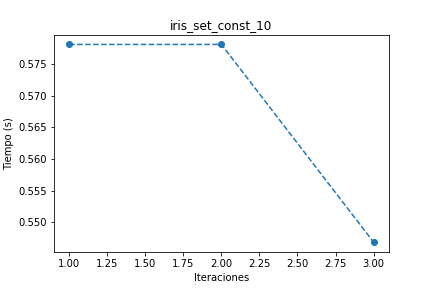
\includegraphics[width=0.234\textwidth]{img/copkm/iris_set_const_10_949004259_time.png}
%     \end{subfigure}
%     \hfill
%     \begin{subfigure}
%         \centering
%         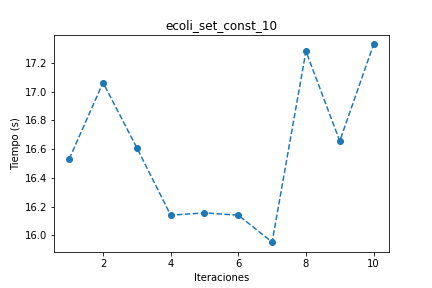
\includegraphics[width=0.234\textwidth]{img/copkm/ecoli_set_const_10_949004259_time.png}
%     \end{subfigure}
%     \hfill
%     \begin{subfigure}
%         \centering
%         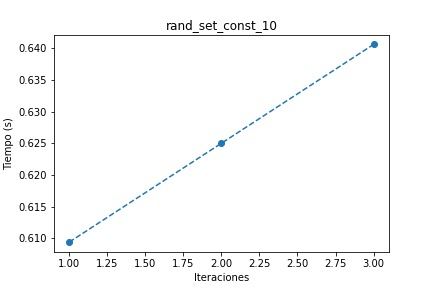
\includegraphics[width=0.234\textwidth]{img/copkm/rand_set_const_10_949004259_time.png}
%     \end{subfigure}
%     \hfill
%     \begin{subfigure}
%         \centering
%         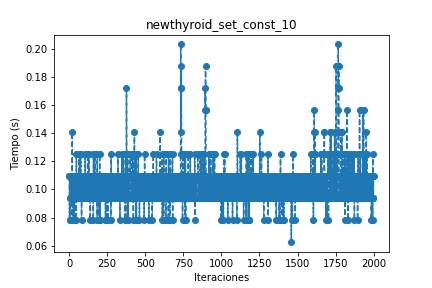
\includegraphics[width=0.234\textwidth]{img/copkm/newthyroid_set_const_10_949004259_time.png}
%     \end{subfigure}
%     \hfill
%     \begin{subfigure}
%         \centering
%         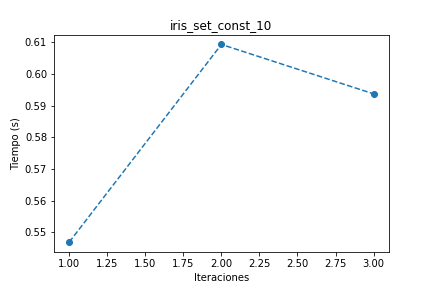
\includegraphics[width=0.234\textwidth]{img/copkm/iris_set_const_10_589741062_time.png}
%     \end{subfigure}
%     \hfill
%     \begin{subfigure}
%         \centering
%         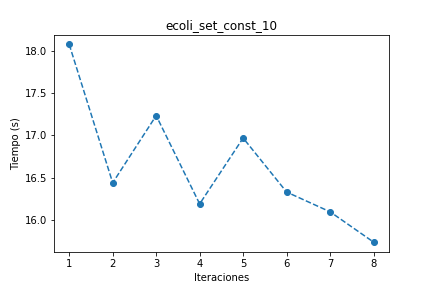
\includegraphics[width=0.234\textwidth]{img/copkm/ecoli_set_const_10_589741062_time.png}
%     \end{subfigure}
%     \hfill
%     \begin{subfigure}
%         \centering
%         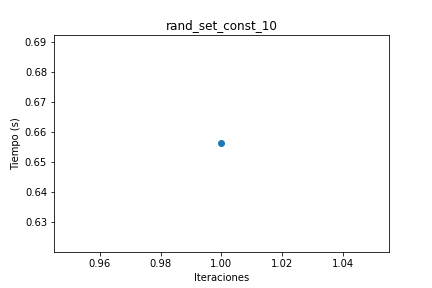
\includegraphics[width=0.234\textwidth]{img/copkm/rand_set_const_10_589741062_time.png}
%     \end{subfigure}
%     \hfill
%     \begin{subfigure}
%         \centering
%         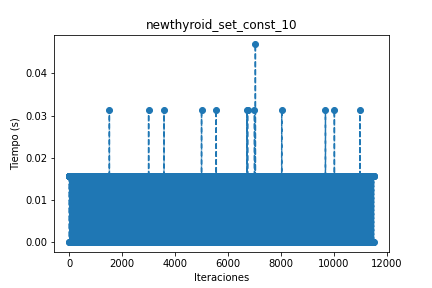
\includegraphics[width=0.234\textwidth]{img/copkm/newthyroid_set_const_10_589741062_time.png}
%     \end{subfigure}
%     \hfill
%     \begin{subfigure}
%         \centering
%         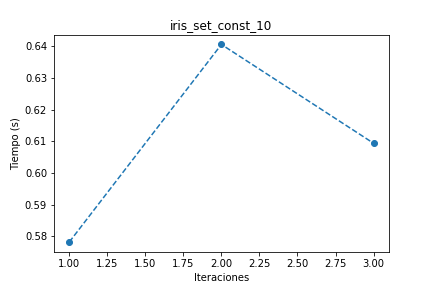
\includegraphics[width=0.234\textwidth]{img/copkm/iris_set_const_10_277451237_time.png}
%     \end{subfigure}
%     \hfill
%     \begin{subfigure}
%         \centering
%         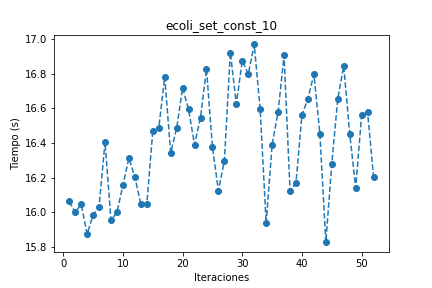
\includegraphics[width=0.234\textwidth]{img/copkm/ecoli_set_const_10_277451237_time.png}
%     \end{subfigure}
%     \hfill
%     \begin{subfigure}
%         \centering
%         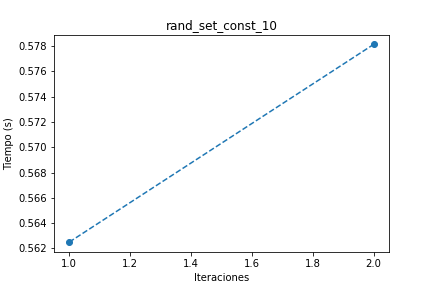
\includegraphics[width=0.234\textwidth]{img/copkm/rand_set_const_10_277451237_time.png}
%     \end{subfigure}
%     \hfill
%     \begin{subfigure}
%         \centering
%         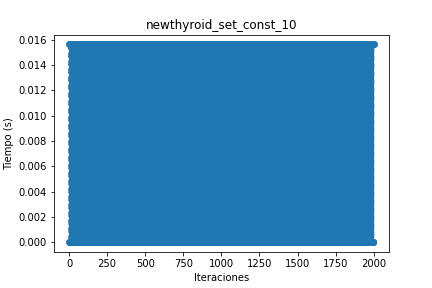
\includegraphics[width=0.234\textwidth]{img/copkm/newthyroid_set_const_10_277451237_time.png}
%     \end{subfigure}
%     \hfill
%     \begin{subfigure}
%         \centering
%         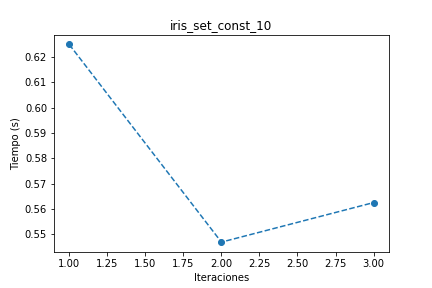
\includegraphics[width=0.234\textwidth]{img/copkm/iris_set_const_10_49258669_time.png}
%     \end{subfigure}
%     \hfill
%     \begin{subfigure}
%         \centering
%         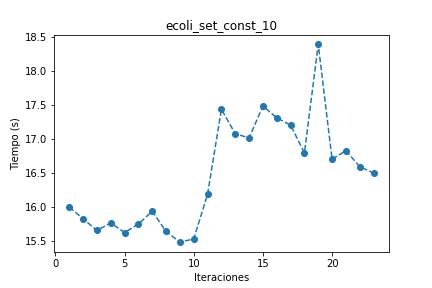
\includegraphics[width=0.234\textwidth]{img/copkm/ecoli_set_const_10_49258669_time.png}
%     \end{subfigure}
%     \hfill
%     \begin{subfigure}
%         \centering
%         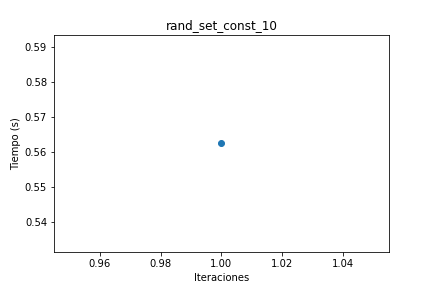
\includegraphics[width=0.234\textwidth]{img/copkm/rand_set_const_10_49258669_time.png}
%     \end{subfigure}
%     \hfill
%     \begin{subfigure}
%         \centering
%         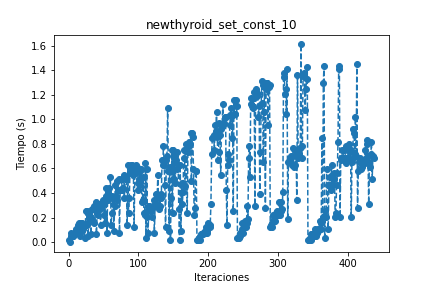
\includegraphics[width=0.234\textwidth]{img/copkm/newthyroid_set_const_10_49258669_time.png}
%     \end{subfigure}
%     \hfill
%     \begin{subfigure}
%         \centering
%         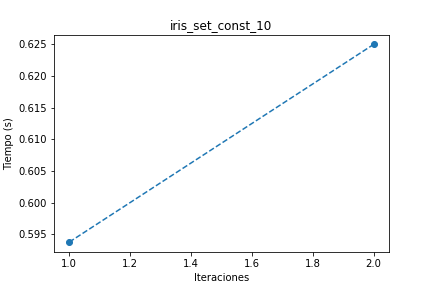
\includegraphics[width=0.234\textwidth]{img/copkm/iris_set_const_10_3773969821_time.png}
%     \end{subfigure}
%     \hfill
%     \begin{subfigure}
%         \centering
%         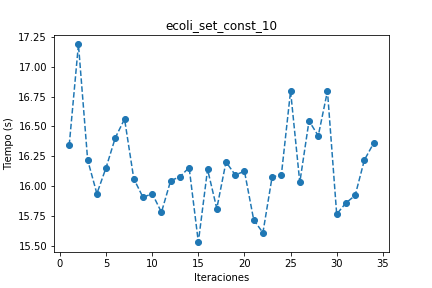
\includegraphics[width=0.234\textwidth]{img/copkm/ecoli_set_const_10_3773969821_time.png}
%     \end{subfigure}
%     \hfill
%     \begin{subfigure}
%         \centering
%         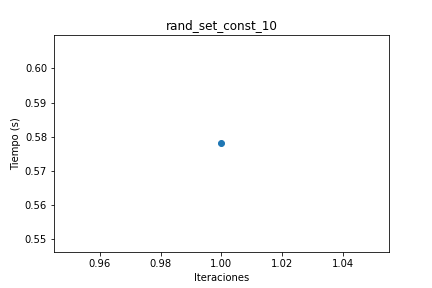
\includegraphics[width=0.234\textwidth]{img/copkm/rand_set_const_10_3773969821_time.png}
%     \end{subfigure}
%     \hfill
%     \begin{subfigure}
%         \centering
%         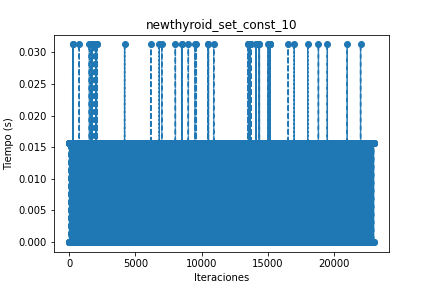
\includegraphics[width=0.234\textwidth]{img/copkm/newthyroid_set_const_10_3773969821_time.png}
%     \end{subfigure}
%     \caption{Tiempos de COPKM v1 para 10\% de restricciones}
% \end{figure}

% \vspace*{\fill}
% \newpage
% \vspace*{\fill}

% \begin{figure}[H]
%     \centering
%     \begin{subfigure}
%         \centering
%         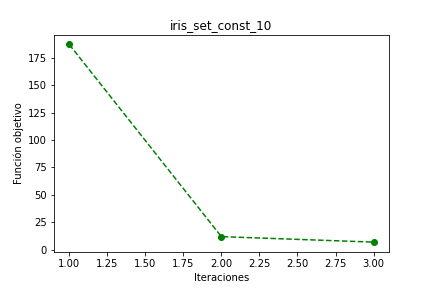
\includegraphics[width=0.234\textwidth]{img/copkm/iris_set_const_10_949004259_cost.png}
%     \end{subfigure}
%     \hfill
%     \begin{subfigure}
%         \centering
%         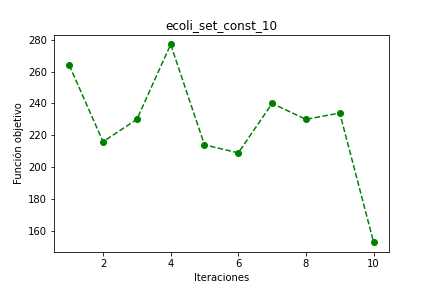
\includegraphics[width=0.234\textwidth]{img/copkm/ecoli_set_const_10_949004259_cost.png}
%     \end{subfigure}
%     \hfill
%     \begin{subfigure}
%         \centering
%         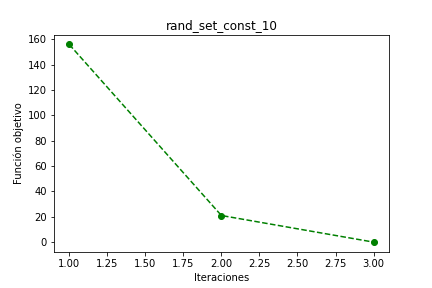
\includegraphics[width=0.234\textwidth]{img/copkm/rand_set_const_10_949004259_cost.png}
%     \end{subfigure}
%     \hfill
%     \begin{subfigure}
%         \centering
%         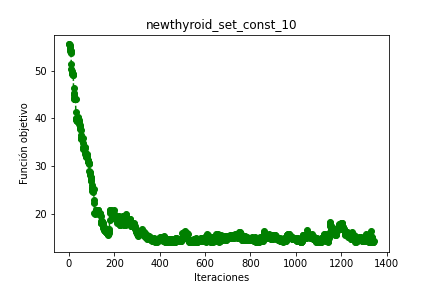
\includegraphics[width=0.234\textwidth]{img/copkm/newthyroid_set_const_10_949004259_cost.png}
%     \end{subfigure}
%     \hfill
%     \begin{subfigure}
%         \centering
%         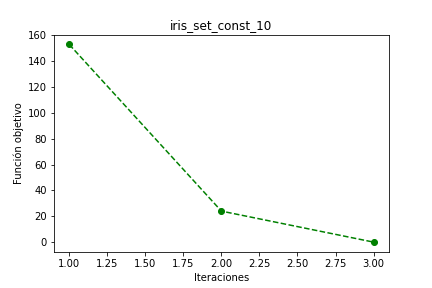
\includegraphics[width=0.234\textwidth]{img/copkm/iris_set_const_10_589741062_cost.png}
%     \end{subfigure}
%     \hfill
%     \begin{subfigure}
%         \centering
%         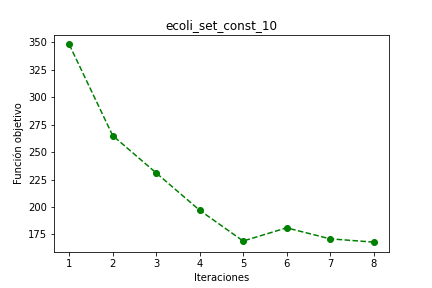
\includegraphics[width=0.234\textwidth]{img/copkm/ecoli_set_const_10_589741062_cost.png}
%     \end{subfigure}
%     \hfill
%     \begin{subfigure}
%         \centering
%         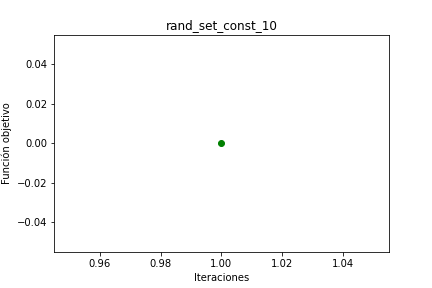
\includegraphics[width=0.234\textwidth]{img/copkm/rand_set_const_10_589741062_cost.png}
%     \end{subfigure}
%     \hfill
%     \begin{subfigure}
%         \centering
%         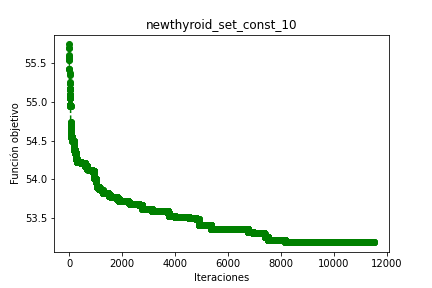
\includegraphics[width=0.234\textwidth]{img/copkm/newthyroid_set_const_10_589741062_cost.png}
%     \end{subfigure}
%     \hfill
%     \begin{subfigure}
%         \centering
%         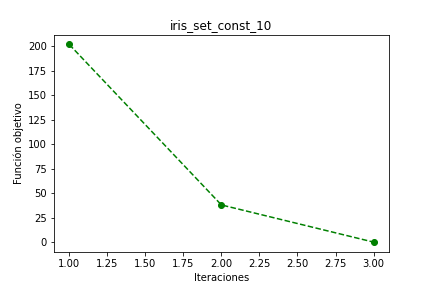
\includegraphics[width=0.234\textwidth]{img/copkm/iris_set_const_10_277451237_cost.png}
%     \end{subfigure}
%     \hfill
%     \begin{subfigure}
%         \centering
%         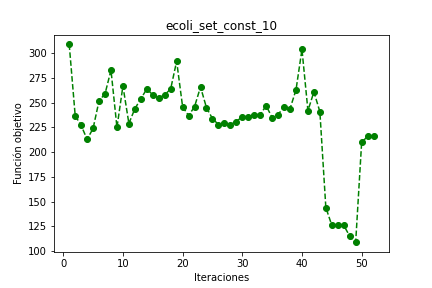
\includegraphics[width=0.234\textwidth]{img/copkm/ecoli_set_const_10_277451237_cost.png}
%     \end{subfigure}
%     \hfill
%     \begin{subfigure}
%         \centering
%         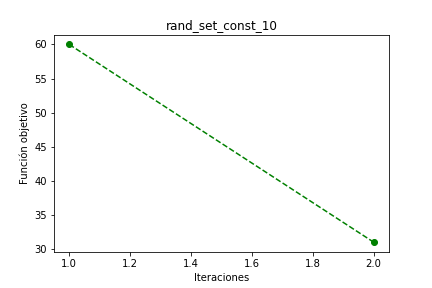
\includegraphics[width=0.234\textwidth]{img/copkm/rand_set_const_10_277451237_cost.png}
%     \end{subfigure}
%     \hfill
%     \begin{subfigure}
%         \centering
%         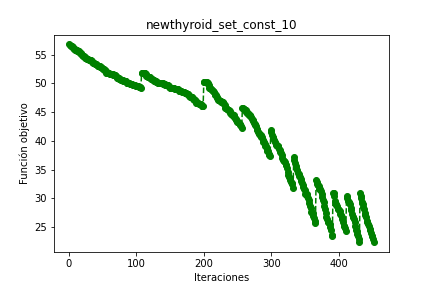
\includegraphics[width=0.234\textwidth]{img/copkm/newthyroid_set_const_10_277451237_cost.png}
%     \end{subfigure}
%     \hfill
%     \begin{subfigure}
%         \centering
%         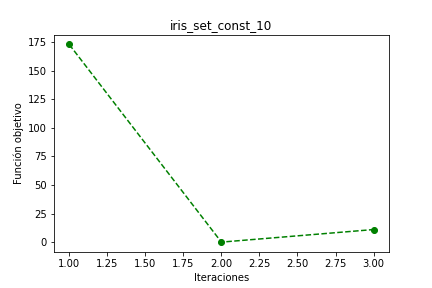
\includegraphics[width=0.234\textwidth]{img/copkm/iris_set_const_10_49258669_cost.png}
%     \end{subfigure}
%     \hfill
%     \begin{subfigure}
%         \centering
%         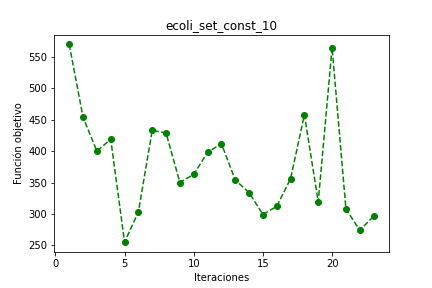
\includegraphics[width=0.234\textwidth]{img/copkm/ecoli_set_const_10_49258669_cost.png}
%     \end{subfigure}
%     \hfill
%     \begin{subfigure}
%         \centering
%         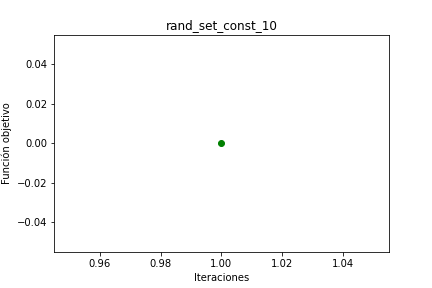
\includegraphics[width=0.234\textwidth]{img/copkm/rand_set_const_10_49258669_cost.png}
%     \end{subfigure}
%     \hfill
%     \begin{subfigure}
%         \centering
%         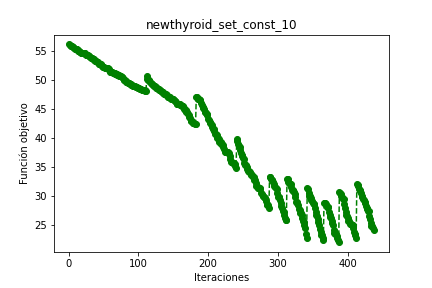
\includegraphics[width=0.234\textwidth]{img/copkm/newthyroid_set_const_10_49258669_cost.png}
%     \end{subfigure}
%     \hfill
%     \begin{subfigure}
%         \centering
%         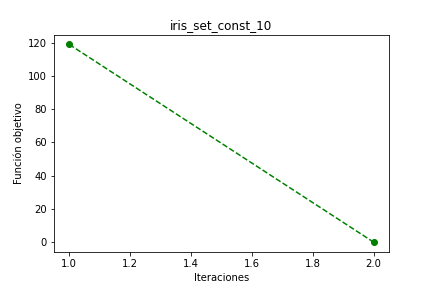
\includegraphics[width=0.234\textwidth]{img/copkm/iris_set_const_10_3773969821_cost.png}
%     \end{subfigure}
%     \hfill
%     \begin{subfigure}
%         \centering
%         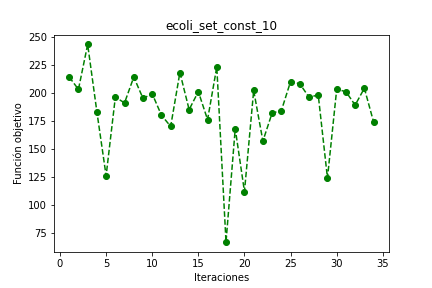
\includegraphics[width=0.234\textwidth]{img/copkm/ecoli_set_const_10_3773969821_cost.png}
%     \end{subfigure}
%     \hfill
%     \begin{subfigure}
%         \centering
%         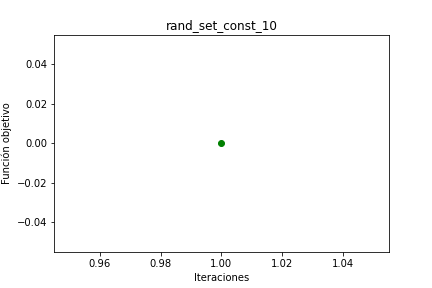
\includegraphics[width=0.234\textwidth]{img/copkm/rand_set_const_10_3773969821_cost.png}
%     \end{subfigure}
%     \hfill
%     \begin{subfigure}
%         \centering
%         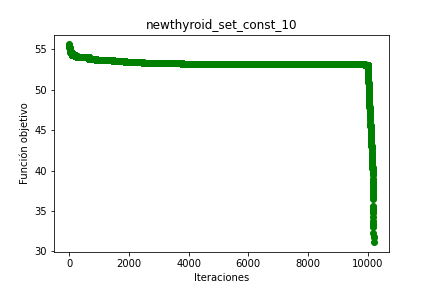
\includegraphics[width=0.234\textwidth]{img/copkm/newthyroid_set_const_10_3773969821_cost.png}
%     \end{subfigure}
%     \caption{Agregado de COPKM v1 para 10\% de restricciones}
% \end{figure}

% % ------------------------------------------------------------------------------

% \vspace*{\fill}

% \newpage

% \vspace*{\fill}

% \begin{table}[H]
%     \centering
%     \resizebox{0.85\columnwidth}{!}{%
%     \makebox[\textwidth][c]{
%         \begin{tabular}{|| c || c c c c || c c c c || c c c c || c c c c ||} 
%             \hline
%             & \multicolumn{4}{|c||}{Iris} & \multicolumn{4}{|c||}{Ecoli} & \multicolumn{4}{|c|}{Rand} & \multicolumn{4}{|c|}{Newthyroid}\\
%             \hline
%             & TasaC & TasaInf & Agr & T & TasaC & TasaInf & Agr & T & TasaC & TasaInf & Agr & T & TasaC & TasaInf & Agr & T \\
%             \hline\hline
%             Ejecución 1 & 0.67 & 17.00 & 0.72 & 3.36 & 34.44 & 351.00 & 39.15 & 169.77 & 0.76 & 0.00 & 0.76 & 3.38 
%             & 14.20 & 67.00 & 15.42 & 10.00
%             \\
%             \hline
%             Ejecución 2 & 0.67 & 0.00 & 0.67 & 2.33 & 37.64 & 158.00 & 39.76 & 283.50 & 0.76 & 0.00 & 0.76 & 2.19 
%             & 14.13 & 30.00 & 14.68 & 9.89
%             \\
%             \hline
%             Ejecución 3 & 0.67 & 0.00 & 0.67 & 5.56 & 33.53 & 128.00 & 35.25 & 366.92 & 0.83 & 68.00 & 1.08 & 3.28 
%             & 14.23 & 60.00 & 15.33 & 9.83
%             \\
%             \hline
%             Ejecución 4 & 0.67 & 0.00 & 0.67 & 3.22 & 32.35 & 92.00 & 33.58 & 392.08 & 0.76 & 0.00 & 0.76 & 2.31 
%             & 14.23 & 30.00 & 14.78 & 13.19
%             \\
%             \hline
%             Ejecución 5 & 0.67 & 0.00 & 0.67 & 3.30 & 37.46 & 118.00 & 39.04 & 158.39 & 0.76 & 0.00 & 0.76 & 2.14 
%             & 14.13 & 14.13 & 15.39 & 9.81
%             \\
%             \hline\hline
%             Media & 0.67 & 3.40 & 0.68 & 3.55 & 35.08 & 169.40 & 37.36 & 274.13 & 0.77 & 13.60 & 0.82 & 2.66 
%             & 14.18 & 40.23 & 15.12 & 10.54
%             \\
%             \hline
%         \end{tabular}
%     }
%     }
%     \caption{Resultados COPKM v1 para 20\% de restricciones}
% \end{table}

% \vspace*{\fill}

% \newpage

% \vspace*{\fill}

% \begin{figure}[H]    
%     \centering
%     \begin{subfigure}
%         \centering
%         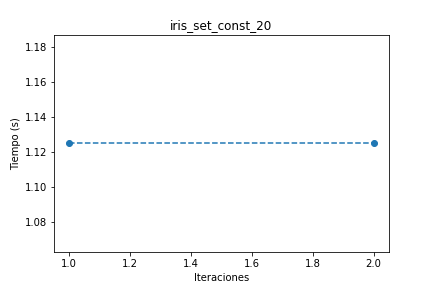
\includegraphics[width=0.234\textwidth]{img/copkm/iris_set_const_20_949004259_time.png}
%     \end{subfigure}
%     \hfill
%     \begin{subfigure}
%         \centering
%         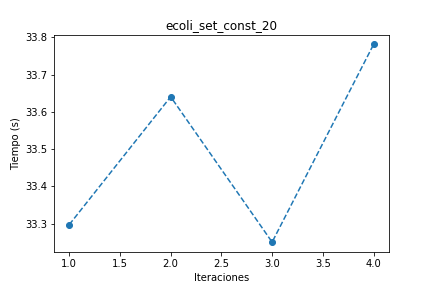
\includegraphics[width=0.234\textwidth]{img/copkm/ecoli_set_const_20_949004259_time.png}
%     \end{subfigure}
%     \hfill
%     \begin{subfigure}
%         \centering
%         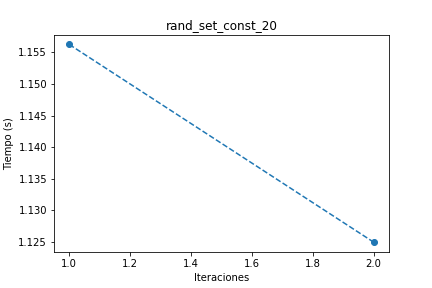
\includegraphics[width=0.234\textwidth]{img/copkm/rand_set_const_20_949004259_time.png}
%     \end{subfigure}
%     \hfill
%     \begin{subfigure}
%         \centering
%         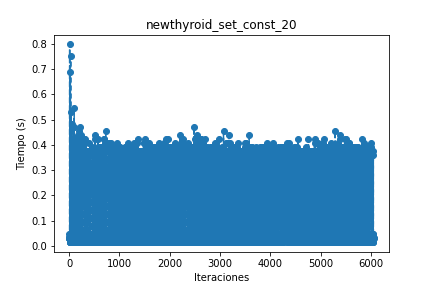
\includegraphics[width=0.234\textwidth]{img/copkm/newthyroid_set_const_20_949004259_time.png}
%     \end{subfigure}
%     \hfill
%     \begin{subfigure}
%         \centering
%         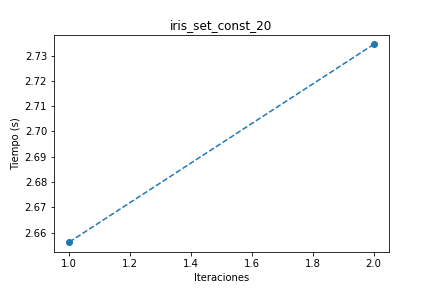
\includegraphics[width=0.234\textwidth]{img/copkm/iris_set_const_20_589741062_time.png}
%     \end{subfigure}
%     \hfill
%     \begin{subfigure}
%         \centering
%         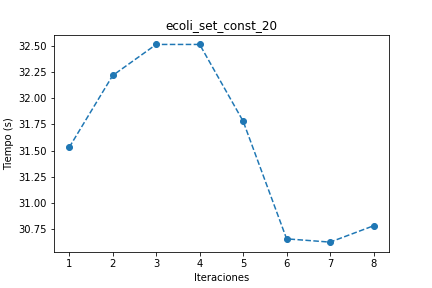
\includegraphics[width=0.234\textwidth]{img/copkm/ecoli_set_const_20_589741062_time.png}
%     \end{subfigure}
%     \hfill
%     \begin{subfigure}
%         \centering
%         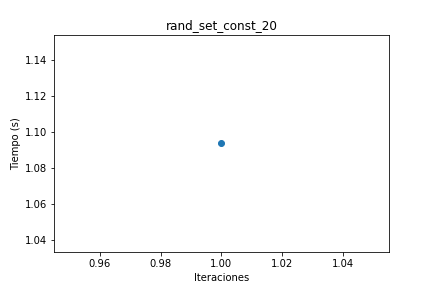
\includegraphics[width=0.234\textwidth]{img/copkm/rand_set_const_20_589741062_time.png}
%     \end{subfigure}
%     \hfill
%     \begin{subfigure}
%         \centering
%         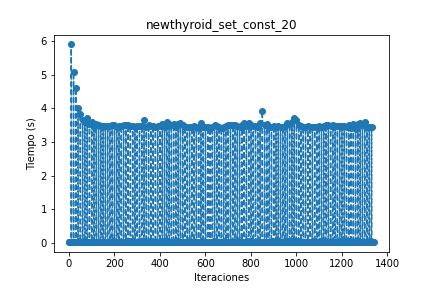
\includegraphics[width=0.234\textwidth]{img/copkm/newthyroid_set_const_20_589741062_time.png}
%     \end{subfigure}
%     \hfill
%     \begin{subfigure}
%         \centering
%         \includegraphics[width=0.234\textwidth]{img/copkm/iris_set_const_20_277451237_time.png}
%     \end{subfigure}
%     \hfill
%     \begin{subfigure}
%         \centering
%         \includegraphics[width=0.234\textwidth]{img/copkm/ecoli_set_const_20_277451237_time.png}
%     \end{subfigure}
%     \hfill
%     \begin{subfigure}
%         \centering
%         \includegraphics[width=0.234\textwidth]{img/copkm/rand_set_const_20_277451237_time.png}
%     \end{subfigure}
%     \hfill
%     \begin{subfigure}
%         \centering
%         \includegraphics[width=0.234\textwidth]{img/copkm/newthyroid_set_const_20_277451237_time.png}
%     \end{subfigure}
%     \hfill
%     \begin{subfigure}
%         \centering
%         \includegraphics[width=0.234\textwidth]{img/copkm/iris_set_const_20_49258669_time.png}
%     \end{subfigure}
%     \hfill
%     \begin{subfigure}
%         \centering
%         \includegraphics[width=0.234\textwidth]{img/copkm/ecoli_set_const_20_49258669_time.png}
%     \end{subfigure}
%     \hfill
%     \begin{subfigure}
%         \centering
%         \includegraphics[width=0.234\textwidth]{img/copkm/rand_set_const_20_49258669_time.png}
%     \end{subfigure}
%     \hfill
%     \begin{subfigure}
%         \centering
%         \includegraphics[width=0.234\textwidth]{img/copkm/newthyroid_set_const_20_49258669_time.png}
%     \end{subfigure}
%     \hfill
%     \begin{subfigure}
%         \centering
%         \includegraphics[width=0.234\textwidth]{img/copkm/iris_set_const_20_3773969821_time.png}
%     \end{subfigure}
%     \hfill
%     \begin{subfigure}
%         \centering
%         \includegraphics[width=0.234\textwidth]{img/copkm/ecoli_set_const_20_3773969821_time.png}
%     \end{subfigure}
%     \hfill
%     \begin{subfigure}
%         \centering
%         \includegraphics[width=0.234\textwidth]{img/copkm/rand_set_const_20_3773969821_time.png}
%     \end{subfigure}
%     \hfill
%     \begin{subfigure}
%         \centering
%         \includegraphics[width=0.234\textwidth]{img/copkm/newthyroid_set_const_20_3773969821_time.png}
%     \end{subfigure}
%     \caption{Tiempos de COPKM v1 para 20\% de restricciones}
% \end{figure}

% \vspace*{\fill}

% \newpage

% \vspace*{\fill}

% \begin{figure}[H]
%     \centering
%     \begin{subfigure}
%         \centering
%         \includegraphics[width=0.234\textwidth]{img/copkm/iris_set_const_20_949004259_cost.png}
%     \end{subfigure}
%     \hfill
%     \begin{subfigure}
%         \centering
%         \includegraphics[width=0.234\textwidth]{img/copkm/ecoli_set_const_20_949004259_cost.png}
%     \end{subfigure}
%     \hfill
%     \begin{subfigure}
%         \centering
%         \includegraphics[width=0.234\textwidth]{img/copkm/rand_set_const_20_949004259_cost.png}
%     \end{subfigure}
%     \hfill
%     \begin{subfigure}
%         \centering
%         \includegraphics[width=0.234\textwidth]{img/copkm/newthyroid_set_const_20_949004259_cost.png}
%     \end{subfigure}
%     \hfill
%     \begin{subfigure}
%         \centering
%         \includegraphics[width=0.234\textwidth]{img/copkm/iris_set_const_20_589741062_cost.png}
%     \end{subfigure}
%     \hfill
%     \begin{subfigure}
%         \centering
%         \includegraphics[width=0.234\textwidth]{img/copkm/ecoli_set_const_20_589741062_cost.png}
%     \end{subfigure}
%     \hfill
%     \begin{subfigure}
%         \centering
%         \includegraphics[width=0.234\textwidth]{img/copkm/rand_set_const_20_589741062_cost.png}
%     \end{subfigure}
%     \hfill
%     \begin{subfigure}
%         \centering
%         \includegraphics[width=0.234\textwidth]{img/copkm/newthyroid_set_const_20_589741062_cost.png}
%     \end{subfigure}
%     \hfill
%     \begin{subfigure}
%         \centering
%         \includegraphics[width=0.234\textwidth]{img/copkm/iris_set_const_20_277451237_cost.png}
%     \end{subfigure}
%     \hfill
%     \begin{subfigure}
%         \centering
%         \includegraphics[width=0.234\textwidth]{img/copkm/ecoli_set_const_20_277451237_cost.png}
%     \end{subfigure}
%     \hfill
%     \begin{subfigure}
%         \centering
%         \includegraphics[width=0.234\textwidth]{img/copkm/rand_set_const_20_277451237_cost.png}
%     \end{subfigure}
%     \hfill
%     \begin{subfigure}
%         \centering
%         \includegraphics[width=0.234\textwidth]{img/copkm/newthyroid_set_const_20_277451237_cost.png}
%     \end{subfigure}
%     \hfill
%     \begin{subfigure}
%         \centering
%         \includegraphics[width=0.234\textwidth]{img/copkm/iris_set_const_20_49258669_cost.png}
%     \end{subfigure}
%     \hfill
%     \begin{subfigure}
%         \centering
%         \includegraphics[width=0.234\textwidth]{img/copkm/ecoli_set_const_20_49258669_cost.png}
%     \end{subfigure}
%     \hfill
%     \begin{subfigure}
%         \centering
%         \includegraphics[width=0.234\textwidth]{img/copkm/rand_set_const_20_49258669_cost.png}
%     \end{subfigure}
%     \hfill
%     \begin{subfigure}
%         \centering
%         \includegraphics[width=0.234\textwidth]{img/copkm/newthyroid_set_const_20_49258669_cost.png}
%     \end{subfigure}
%     \hfill
%     \begin{subfigure}
%         \centering
%         \includegraphics[width=0.234\textwidth]{img/copkm/iris_set_const_20_3773969821_cost.png}
%     \end{subfigure}
%     \hfill
%     \begin{subfigure}
%         \centering
%         \includegraphics[width=0.234\textwidth]{img/copkm/ecoli_set_const_20_3773969821_cost.png}
%     \end{subfigure}
%     \hfill
%     \begin{subfigure}
%         \centering
%         \includegraphics[width=0.234\textwidth]{img/copkm/rand_set_const_20_3773969821_cost.png}
%     \end{subfigure}
%     \hfill
%     \begin{subfigure}
%         \centering
%         \includegraphics[width=0.234\textwidth]{img/copkm/newthyroid_set_const_20_3773969821_cost.png}
%     \end{subfigure}
%     \caption{Agregado de COPKM v1 para 20\% de restricciones}
% \end{figure}

% \vspace*{\fill}

% \newpage

% \subsection{Búsqueda Local}

% En todas las ejecuciones se utilizó un valor $\lambda$ igual al cociente entre la mayor distancia entre dos elementos cualesquiera del conjunto de datos y el número de restricciones del problema.

% \begin{equation}    
%     \lambda = \frac{\max D}{|R|}
% \end{equation}

% \vspace{\baselineskip}

% % Gráfica con consume de tiempo por ciclo

% \vspace*{\fill}

% \begin{table}[H]
%     \centering
%     \resizebox{0.85\columnwidth}{!}{%
%     \makebox[\textwidth][c]{
%         \begin{tabular}{|| c || c c c c || c c c c || c c c c || c c c c ||} 
%             \hline
%             & \multicolumn{4}{|c||}{Iris} & \multicolumn{4}{|c||}{Ecoli} & \multicolumn{4}{|c|}{Rand} & \multicolumn{4}{|c|}{Newthyroid}\\
%             \hline
%             & TasaC & TasaInf & Agr & T & TasaC & TasaInf & Agr & T & TasaC & TasaInf & Agr & T & TasaC & TasaInf & Agr & T \\
%             \hline\hline
%             Ejecución 1 & 1.07 & 241.00 & 2.60 & 17.27 & 46.46 & 1188.00 & 78.34 & 747.25 & 1.22 & 131.00 & 2.17 & 27.70 
%             & 14.87 & 271.00 & 24.78 & 157.25
%             \\
%             \hline
%             Ejecución 2 & 1.02 & 193.00 & 2.24 & 20.77 & 46.63 & 1207.00 & 79.01 & 712.41 & 1.23 & 133.00 & 2.19 & 21.05 
%             & 14.27 & 221.00 & 22.36 & 128.27
%             \\
%             \hline
%             Ejecución 3 & 1.02 & 133.00 & 1.86 & 30.67 & 46.63 & 1228.00 & 79.58 & 741.86 & 1.14 & 133.00 & 2.10 & 35.20 
%             & 14.40 & 388.00 & 28.59 & 122.80
%             \\
%             \hline
%             Ejecución 4 & 0.76 & 75.00 & 1.23 & 29.66 & 47.39 & 1197.00 & 79.50 & 753.13 & 1.04 & 78.00 & 1.61 & 29.38 
%             & 13.05 & 302.00 & 24.10 & 141.84
%             \\
%             \hline
%             Ejecución 5 & 0.76 & 64.00 & 1.16 & 39.13 & 46.60 & 1244.00 & 79.98 & 712.03 & 0.95 & 55.00 & 1.35 & 32.73 
%             & 14.22 & 302.00 & 25.27 & 110.33
%             \\
%             \hline\hline
%             Media & 0.92 & 141.20 & 1.82 & 27.50 & 46.74 & 1212.80 & 79.28 & 733.33 & 1.12 & 106.00 & 1.88 & 29.21 
%             & 14.16 & 296.80 & 25.02 & 132.10
%             \\
%             \hline
%         \end{tabular}
%     }
%     }
%     \caption{Resultados BL para 10\% de restricciones}
% \end{table}

% \vspace*{\fill}
% \newpage
% \vspace*{\fill}

% \begin{figure}[H]
%     \centering
%     \begin{subfigure}
%         \centering
%         \includegraphics[width=0.234\textwidth]{img/bl/iris_set_const_10_949004259_time.png}
%     \end{subfigure}
%     \hfill
%     \begin{subfigure}
%         \centering
%         \includegraphics[width=0.234\textwidth]{img/bl/ecoli_set_const_10_949004259_time.png}
%     \end{subfigure}
%     \hfill
%     \begin{subfigure}
%         \centering
%         \includegraphics[width=0.234\textwidth]{img/bl/rand_set_const_10_949004259_time.png}
%     \end{subfigure}
%     \hfill
%     \begin{subfigure}
%         \centering
%         \includegraphics[width=0.234\textwidth]{img/bl/newthyroid_set_const_10_949004259_time.png}
%     \end{subfigure}
%     \hfill
%     \begin{subfigure}
%         \centering
%         \includegraphics[width=0.234\textwidth]{img/bl/iris_set_const_10_589741062_time.png}
%     \end{subfigure}
%     \hfill
%     \begin{subfigure}
%         \centering
%         \includegraphics[width=0.234\textwidth]{img/bl/ecoli_set_const_10_589741062_time.png}
%     \end{subfigure}
%     \hfill
%     \begin{subfigure}
%         \centering
%         \includegraphics[width=0.234\textwidth]{img/bl/rand_set_const_10_589741062_time.png}
%     \end{subfigure}
%     \hfill
%     \begin{subfigure}
%         \centering
%         \includegraphics[width=0.234\textwidth]{img/bl/newthyroid_set_const_10_589741062_time.png}
%     \end{subfigure}
%     \hfill
%     \begin{subfigure}
%         \centering
%         \includegraphics[width=0.234\textwidth]{img/bl/iris_set_const_10_277451237_time.png}
%     \end{subfigure}
%     \hfill
%     \begin{subfigure}
%         \centering
%         \includegraphics[width=0.234\textwidth]{img/bl/ecoli_set_const_10_277451237_time.png}
%     \end{subfigure}
%     \hfill
%     \begin{subfigure}
%         \centering
%         \includegraphics[width=0.234\textwidth]{img/bl/rand_set_const_10_277451237_time.png}
%     \end{subfigure}
%     \hfill
%     \begin{subfigure}
%         \centering
%         \includegraphics[width=0.234\textwidth]{img/bl/newthyroid_set_const_10_277451237_time.png}
%     \end{subfigure}
%     \hfill
%     \begin{subfigure}
%         \centering
%         \includegraphics[width=0.234\textwidth]{img/bl/iris_set_const_10_49258669_time.png}
%     \end{subfigure}
%     \hfill
%     \begin{subfigure}
%         \centering
%         \includegraphics[width=0.234\textwidth]{img/bl/ecoli_set_const_10_49258669_time.png}
%     \end{subfigure}
%     \hfill
%     \begin{subfigure}
%         \centering
%         \includegraphics[width=0.234\textwidth]{img/bl/rand_set_const_10_49258669_time.png}
%     \end{subfigure}
%     \hfill
%     \begin{subfigure}
%         \centering
%         \includegraphics[width=0.234\textwidth]{img/bl/newthyroid_set_const_10_49258669_time.png}
%     \end{subfigure}
%     \hfill
%     \begin{subfigure}
%         \centering
%         \includegraphics[width=0.234\textwidth]{img/bl/iris_set_const_10_3773969821_time.png}
%     \end{subfigure}
%     \hfill
%     \begin{subfigure}
%         \centering
%         \includegraphics[width=0.234\textwidth]{img/bl/ecoli_set_const_10_3773969821_time.png}
%     \end{subfigure}
%     \hfill
%     \begin{subfigure}
%         \centering
%         \includegraphics[width=0.234\textwidth]{img/bl/rand_set_const_10_3773969821_time.png}
%     \end{subfigure}
%     \hfill
%     \begin{subfigure}
%         \centering
%         \includegraphics[width=0.234\textwidth]{img/bl/newthyroid_set_const_10_3773969821_time.png}
%     \end{subfigure}
%     \caption{Tiempos de BL para 10\% de restricciones}
% \end{figure}

% \vspace*{\fill}
% \newpage
% \vspace*{\fill}

% \begin{figure}[H]
%     \centering
%     \begin{subfigure}
%         \centering
%         \includegraphics[width=0.234\textwidth]{img/bl/iris_set_const_10_949004259_cost.png}
%     \end{subfigure}
%     \hfill
%     \begin{subfigure}
%         \centering
%         \includegraphics[width=0.234\textwidth]{img/bl/ecoli_set_const_10_949004259_cost.png}
%     \end{subfigure}
%     \hfill
%     \begin{subfigure}
%         \centering
%         \includegraphics[width=0.234\textwidth]{img/bl/rand_set_const_10_949004259_cost.png}
%     \end{subfigure}
%     \hfill
%     \begin{subfigure}
%         \centering
%         \includegraphics[width=0.234\textwidth]{img/bl/newthyroid_set_const_10_949004259_cost.png}
%     \end{subfigure}
%     \hfill
%     \begin{subfigure}
%         \centering
%         \includegraphics[width=0.234\textwidth]{img/bl/iris_set_const_10_589741062_cost.png}
%     \end{subfigure}
%     \hfill
%     \begin{subfigure}
%         \centering
%         \includegraphics[width=0.234\textwidth]{img/bl/ecoli_set_const_10_589741062_cost.png}
%     \end{subfigure}
%     \hfill
%     \begin{subfigure}
%         \centering
%         \includegraphics[width=0.234\textwidth]{img/bl/rand_set_const_10_589741062_cost.png}
%     \end{subfigure}
%     \hfill
%     \begin{subfigure}
%         \centering
%         \includegraphics[width=0.234\textwidth]{img/bl/newthyroid_set_const_10_589741062_cost.png}
%     \end{subfigure}
%     \hfill
%     \begin{subfigure}
%         \centering
%         \includegraphics[width=0.234\textwidth]{img/bl/iris_set_const_10_277451237_cost.png}
%     \end{subfigure}
%     \hfill
%     \begin{subfigure}
%         \centering
%         \includegraphics[width=0.234\textwidth]{img/bl/ecoli_set_const_10_277451237_cost.png}
%     \end{subfigure}
%     \hfill
%     \begin{subfigure}
%         \centering
%         \includegraphics[width=0.234\textwidth]{img/bl/rand_set_const_10_277451237_cost.png}
%     \end{subfigure}
%     \hfill
%     \begin{subfigure}
%         \centering
%         \includegraphics[width=0.234\textwidth]{img/bl/newthyroid_set_const_10_277451237_cost.png}
%     \end{subfigure}
%     \hfill
%     \begin{subfigure}
%         \centering
%         \includegraphics[width=0.234\textwidth]{img/bl/iris_set_const_10_49258669_cost.png}
%     \end{subfigure}
%     \hfill
%     \begin{subfigure}
%         \centering
%         \includegraphics[width=0.234\textwidth]{img/bl/ecoli_set_const_10_49258669_cost.png}
%     \end{subfigure}
%     \hfill
%     \begin{subfigure}
%         \centering
%         \includegraphics[width=0.234\textwidth]{img/bl/rand_set_const_10_49258669_cost.png}
%     \end{subfigure}
%     \hfill
%     \begin{subfigure}
%         \centering
%         \includegraphics[width=0.234\textwidth]{img/bl/newthyroid_set_const_10_49258669_cost.png}
%     \end{subfigure}
%     \hfill
%     \begin{subfigure}
%         \centering
%         \includegraphics[width=0.234\textwidth]{img/bl/iris_set_const_10_3773969821_cost.png}
%     \end{subfigure}
%     \hfill
%     \begin{subfigure}
%         \centering
%         \includegraphics[width=0.234\textwidth]{img/bl/ecoli_set_const_10_3773969821_cost.png}
%     \end{subfigure}
%     \hfill
%     \begin{subfigure}
%         \centering
%         \includegraphics[width=0.234\textwidth]{img/bl/rand_set_const_10_3773969821_cost.png}
%     \end{subfigure}
%     \hfill
%     \begin{subfigure}
%         \centering
%         \includegraphics[width=0.234\textwidth]{img/bl/newthyroid_set_const_10_3773969821_cost.png}
%     \end{subfigure}
%     \caption{Agregado de BL para 10\% de restricciones}
% \end{figure}

% \vspace*{\fill}
% \newpage
% \vspace*{\fill}

% \begin{table}[H]
%     \centering
%     \resizebox{0.85\columnwidth}{!}{%
%     \makebox[\textwidth][c]{
%         \begin{tabular}{|| c || c c c c || c c c c || c c c c || c c c c ||} 
%             \hline
%             & \multicolumn{4}{|c||}{Iris} & \multicolumn{4}{|c||}{Ecoli} & \multicolumn{4}{|c|}{Rand} & \multicolumn{4}{|c|}{Newthyroid}\\
%             \hline
%             & TasaC & TasaInf & Agr & T & TasaC & TasaInf & Agr & T & TasaC & TasaInf & Agr & T & TasaC & TasaInf & Agr & T \\
%             \hline\hline
%             Ejecución 1 & 0.82 & 279.00 & 1.70 & 42.30 & 46.28 & 2133.00 & 74.89 & 1256.20 & 1.14 & 272.00 & 2.12 & 40.48 
%             & 14.82 & 602.00 & 25.83 & 235.84
%             \\
%             \hline
%             Ejecución 2 & 0.94 & 325.00 & 1.97 & 32.75 & 46.64 & 2194.00 & 76.07 & 1220.25 & 1.25 & 366.00 & 2.57 & 33.13 
%             & 14.83 & 519.00 & 24.31 & 159.41
%             \\
%             \hline
%             Ejecución 3 & 1.11 & 338.00 & 2.18 & 36.50 & 46.88 & 2178.00 & 76.10 & 1234.64 & 1.07 & 258.00 & 2.00 & 40.19 
%             & 14.37 & 597.00 & 25.29 & 175.42
%             \\
%             \hline
%             Ejecución 4 & 0.93 & 276.00 & 1.80 & 38.41 & 47.14 & 2190.00 & 76.52 & 1223.83 & 1.02 & 194.00 & 1.71 & 44.39 
%             & 14.10 & 610.00 & 25.25 & 170.97
%             \\
%             \hline
%             Ejecución 5 & 0.72 & 106.00 & 1.05 & 50.94 & 47.30 & 2181.00 & 76.56 & 1277.31 & 1.30 & 376.00 & 2.65 & 33.05  & 14.61 & 553.00 & 24.72 & 170.14
%             \\
%             \hline\hline
%             Media & 0.90 & 264.80 & 1.74 & 40.18 & 46.85 & 2175.20 & 76.03 & 1242.45 & 1.15 & 293.20 & 2.21 & 38.25  & 14.54 & 576.20 & 25.08 & 182.36 \\
%             \hline

%         \end{tabular}
%     }   
%     }
%     \caption{Resultados BL para 20\% de restricciones}
% \end{table}

% \vspace*{\fill}
% \newpage
% \vspace*{\fill}

% \begin{figure}[H]    
%     \centering
%     \begin{subfigure}
%         \centering
%         \includegraphics[width=0.234\textwidth]{img/bl/iris_set_const_20_949004259_time.png}
%     \end{subfigure}
%     \hfill
%     \begin{subfigure}
%         \centering
%         \includegraphics[width=0.234\textwidth]{img/bl/ecoli_set_const_20_949004259_time.png}
%     \end{subfigure}
%     \hfill
%     \begin{subfigure}
%         \centering
%         \includegraphics[width=0.234\textwidth]{img/bl/rand_set_const_20_949004259_time.png}
%     \end{subfigure}
%     \hfill
%     \begin{subfigure}
%         \centering
%         \includegraphics[width=0.234\textwidth]{img/bl/newthyroid_set_const_20_949004259_time.png}
%     \end{subfigure}
%     \hfill
%     \begin{subfigure}
%         \centering
%         \includegraphics[width=0.234\textwidth]{img/bl/iris_set_const_20_589741062_time.png}
%     \end{subfigure}
%     \hfill
%     \begin{subfigure}
%         \centering
%         \includegraphics[width=0.234\textwidth]{img/bl/ecoli_set_const_20_589741062_time.png}
%     \end{subfigure}
%     \hfill
%     \begin{subfigure}
%         \centering
%         \includegraphics[width=0.234\textwidth]{img/bl/rand_set_const_20_589741062_time.png}
%     \end{subfigure}
%     \hfill
%     \begin{subfigure}
%         \centering
%         \includegraphics[width=0.234\textwidth]{img/bl/newthyroid_set_const_20_589741062_time.png}
%     \end{subfigure}
%     \hfill
%     \begin{subfigure}
%         \centering
%         \includegraphics[width=0.234\textwidth]{img/bl/iris_set_const_20_277451237_time.png}
%     \end{subfigure}
%     \hfill
%     \begin{subfigure}
%         \centering
%         \includegraphics[width=0.234\textwidth]{img/bl/ecoli_set_const_20_277451237_time.png}
%     \end{subfigure}
%     \hfill
%     \begin{subfigure}
%         \centering
%         \includegraphics[width=0.234\textwidth]{img/bl/rand_set_const_20_277451237_time.png}
%     \end{subfigure}
%     \hfill
%     \begin{subfigure}
%         \centering
%         \includegraphics[width=0.234\textwidth]{img/bl/newthyroid_set_const_20_277451237_time.png}
%     \end{subfigure}
%     \hfill
%     \begin{subfigure}
%         \centering
%         \includegraphics[width=0.234\textwidth]{img/bl/iris_set_const_20_49258669_time.png}
%     \end{subfigure}
%     \hfill
%     \begin{subfigure}
%         \centering
%         \includegraphics[width=0.234\textwidth]{img/bl/ecoli_set_const_20_49258669_time.png}
%     \end{subfigure}
%     \hfill
%     \begin{subfigure}
%         \centering
%         \includegraphics[width=0.234\textwidth]{img/bl/rand_set_const_20_49258669_time.png}
%     \end{subfigure}
%     \hfill
%     \begin{subfigure}
%         \centering
%         \includegraphics[width=0.234\textwidth]{img/bl/newthyroid_set_const_20_49258669_time.png}
%     \end{subfigure}
%     \hfill
%     \begin{subfigure}
%         \centering
%         \includegraphics[width=0.234\textwidth]{img/bl/iris_set_const_20_3773969821_time.png}
%     \end{subfigure}
%     \hfill
%     \begin{subfigure}
%         \centering
%         \includegraphics[width=0.234\textwidth]{img/bl/ecoli_set_const_20_3773969821_time.png}
%     \end{subfigure}
%     \hfill
%     \begin{subfigure}
%         \centering
%         \includegraphics[width=0.234\textwidth]{img/bl/rand_set_const_20_3773969821_time.png}
%     \end{subfigure}
%     \hfill
%     \begin{subfigure}
%         \centering
%         \includegraphics[width=0.234\textwidth]{img/bl/newthyroid_set_const_20_3773969821_time.png}
%     \end{subfigure}
%     \caption{Tiempos de BL para 20\% de restricciones}
% \end{figure}

% \vspace*{\fill}
% \newpage
% \vspace*{\fill}

% \begin{figure}[H]
%     \centering
%     \begin{subfigure}
%         \centering
%         \includegraphics[width=0.234\textwidth]{img/bl/iris_set_const_20_949004259_cost.png}
%     \end{subfigure}
%     \hfill
%     \begin{subfigure}
%         \centering
%         \includegraphics[width=0.234\textwidth]{img/bl/ecoli_set_const_20_949004259_cost.png}
%     \end{subfigure}
%     \hfill
%     \begin{subfigure}
%         \centering
%         \includegraphics[width=0.234\textwidth]{img/bl/rand_set_const_20_949004259_cost.png}
%     \end{subfigure}
%     \hfill
%     \begin{subfigure}
%         \centering
%         \includegraphics[width=0.234\textwidth]{img/bl/newthyroid_set_const_20_949004259_cost.png}
%     \end{subfigure}
%     \hfill
%     \begin{subfigure}
%         \centering
%         \includegraphics[width=0.234\textwidth]{img/bl/iris_set_const_20_589741062_cost.png}
%     \end{subfigure}
%     \hfill
%     \begin{subfigure}
%         \centering
%         \includegraphics[width=0.234\textwidth]{img/bl/ecoli_set_const_20_589741062_cost.png}
%     \end{subfigure}
%     \hfill
%     \begin{subfigure}
%         \centering
%         \includegraphics[width=0.234\textwidth]{img/bl/rand_set_const_20_589741062_cost.png}
%     \end{subfigure}
%     \hfill
%     \begin{subfigure}
%         \centering
%         \includegraphics[width=0.234\textwidth]{img/bl/newthyroid_set_const_20_589741062_cost.png}
%     \end{subfigure}
%     \hfill
%     \begin{subfigure}
%         \centering
%         \includegraphics[width=0.234\textwidth]{img/bl/iris_set_const_20_277451237_cost.png}
%     \end{subfigure}
%     \hfill
%     \begin{subfigure}
%         \centering
%         \includegraphics[width=0.234\textwidth]{img/bl/ecoli_set_const_20_277451237_cost.png}
%     \end{subfigure}
%     \hfill
%     \begin{subfigure}
%         \centering
%         \includegraphics[width=0.234\textwidth]{img/bl/rand_set_const_20_277451237_cost.png}
%     \end{subfigure}
%     \hfill
%     \begin{subfigure}
%         \centering
%         \includegraphics[width=0.234\textwidth]{img/bl/newthyroid_set_const_20_277451237_cost.png}
%     \end{subfigure}
%     \hfill
%     \begin{subfigure}
%         \centering
%         \includegraphics[width=0.234\textwidth]{img/bl/iris_set_const_20_49258669_cost.png}
%     \end{subfigure}
%     \hfill
%     \begin{subfigure}
%         \centering
%         \includegraphics[width=0.234\textwidth]{img/bl/ecoli_set_const_20_49258669_cost.png}
%     \end{subfigure}
%     \hfill
%     \begin{subfigure}
%         \centering
%         \includegraphics[width=0.234\textwidth]{img/bl/rand_set_const_20_49258669_cost.png}
%     \end{subfigure}
%     \hfill
%     \begin{subfigure}
%         \centering
%         \includegraphics[width=0.234\textwidth]{img/bl/newthyroid_set_const_20_49258669_cost.png}
%     \end{subfigure}
%     \hfill
%     \begin{subfigure}
%         \centering
%         \includegraphics[width=0.234\textwidth]{img/bl/iris_set_const_20_3773969821_cost.png}
%     \end{subfigure}
%     \hfill
%     \begin{subfigure}
%         \centering
%         \includegraphics[width=0.234\textwidth]{img/bl/ecoli_set_const_20_3773969821_cost.png}
%     \end{subfigure}
%     \hfill
%     \begin{subfigure}
%         \centering
%         \includegraphics[width=0.234\textwidth]{img/bl/rand_set_const_20_3773969821_cost.png}
%     \end{subfigure}
%     \hfill
%     \begin{subfigure}
%         \centering
%         \includegraphics[width=0.234\textwidth]{img/bl/newthyroid_set_const_20_3773969821_cost.png}
%     \end{subfigure}
%     \caption{Agregado de BL para 20\% de restricciones}
% \end{figure}

% \vspace*{\fill}
% \newpage

% \subsection{Greedy COPKM v2}

% \vspace*{\fill}

% \begin{table}[H]
%     \centering
%     \resizebox{0.85\columnwidth}{!}{%
%     \makebox[\textwidth][c]{
%         \begin{tabular}{|| c || c c c c || c c c c || c c c c || c c c c ||} 
%             \hline
%             & \multicolumn{4}{|c||}{Iris} & \multicolumn{4}{|c||}{Ecoli} & \multicolumn{4}{|c|}{Rand} & \multicolumn{4}{|c|}{Newthyroid}\\
%             \hline
%             & TasaC & TasaInf & Agr & T & TasaC & TasaInf & Agr & T & TasaC & TasaInf & Agr & T & TasaC & TasaInf & Agr & T \\
%             \hline\hline
%             Ejecución 1 & 0.67 & 0.00 & 0.67 & 2.11 & 34.74 & 2.00 & 34.80 & 89.83 & 0.76 & 0.00 & 0.76 & 2.25 & 14.29 & 0.00 & 14.29 & 6.23 \\
%             \hline
%             Ejecución 2 & 0.67 & 0.00 & 0.67 & 2.72 & 29.37 & 0.00 & 29.37 & 152.09 & 0.76 & 0.00 & 0.76 & 1.66 & 14.29 & 0.00 & 14.29 & 6.39\\
%             \hline
%             Ejecución 3 & 0.67 & 0.00 & 0.67 & 2.89 & 57.53 & 277.00 & 64.96 & 59.25 & 0.76 & 0.00 & 0.76 & 2.27 & 14.29 & 0.00 & 14.29 & 8.56\\
%             \hline
%             Ejecución 4 & 0.67 & 0.00 & 0.67 & 2.22 & 33.71 & 4.00 & 33.71 & 106.02 & 0.76 & 0.00 & 0.76 & 1.69  & 14.29 & 0.00 & 14.29 & 6.97\\
%             \hline
%             Ejecución 5 & 0.67 & 0.00 & 0.67 & 2.25 & 32.15 & 3.00 & 32.23 & 182.00 & 0.76 & 0.00 & 0.76 & 2.25 & 14.29 & 0.00 & 14.29 & 6.22\\
%             \hline\hline
%             Media & 0.67 & 0.00 & 0.67 & 2.44 & 37.50 & 57.20 & 39.01 & 117.84 & 0.76 & 0.00 & 0.76 & 2.02 & 14.29 & 0.00 & 14.29 & 6.88 \\
%             \hline

%         \end{tabular}
%     }
%     }
%     \caption{Resultados de COPKM v2 para 10\% de restricciones}
% \end{table}

% \vspace*{\fill}
% \newpage
% \vspace*{\fill}

% \begin{figure}[H]    
%     \centering
%     \begin{subfigure}
%         \centering
%         \includegraphics[width=0.234\textwidth]{img/copkm2/iris_set_const_10_949004259_time.png}
%     \end{subfigure}
%     \hfill
%     \begin{subfigure}
%         \centering
%         \includegraphics[width=0.234\textwidth]{img/copkm2/ecoli_set_const_10_949004259_time.png}
%     \end{subfigure}
%     \hfill
%     \begin{subfigure}
%         \centering
%         \includegraphics[width=0.234\textwidth]{img/copkm2/rand_set_const_10_949004259_time.png}
%     \end{subfigure}
%     \hfill
%     \begin{subfigure}
%         \centering
%         \includegraphics[width=0.234\textwidth]{img/copkm2/newthyroid_set_const_10_949004259_time.png}
%     \end{subfigure}
%     \hfill
%     \begin{subfigure}
%         \centering
%         \includegraphics[width=0.234\textwidth]{img/copkm2/iris_set_const_10_589741062_time.png}
%     \end{subfigure}
%     \hfill
%     \begin{subfigure}
%         \centering
%         \includegraphics[width=0.234\textwidth]{img/copkm2/ecoli_set_const_10_589741062_time.png}
%     \end{subfigure}
%     \hfill
%     \begin{subfigure}
%         \centering
%         \includegraphics[width=0.234\textwidth]{img/copkm2/rand_set_const_10_589741062_time.png}
%     \end{subfigure}
%     \hfill
%     \begin{subfigure}
%         \centering
%         \includegraphics[width=0.234\textwidth]{img/copkm2/newthyroid_set_const_10_589741062_time.png}
%     \end{subfigure}
%     \hfill
%     \begin{subfigure}
%         \centering
%         \includegraphics[width=0.234\textwidth]{img/copkm2/iris_set_const_10_277451237_time.png}
%     \end{subfigure}
%     \hfill
%     \begin{subfigure}
%         \centering
%         \includegraphics[width=0.234\textwidth]{img/copkm2/ecoli_set_const_10_277451237_time.png}
%     \end{subfigure}
%     \hfill
%     \begin{subfigure}
%         \centering
%         \includegraphics[width=0.234\textwidth]{img/copkm2/rand_set_const_10_277451237_time.png}
%     \end{subfigure}
%     \hfill
%     \begin{subfigure}
%         \centering
%         \includegraphics[width=0.234\textwidth]{img/copkm2/newthyroid_set_const_10_277451237_time.png}
%     \end{subfigure}
%     \hfill
%     \begin{subfigure}
%         \centering
%         \includegraphics[width=0.234\textwidth]{img/copkm2/iris_set_const_10_49258669_time.png}
%     \end{subfigure}
%     \hfill
%     \begin{subfigure}
%         \centering
%         \includegraphics[width=0.234\textwidth]{img/copkm2/ecoli_set_const_10_49258669_time.png}
%     \end{subfigure}
%     \hfill
%     \begin{subfigure}
%         \centering
%         \includegraphics[width=0.234\textwidth]{img/copkm2/rand_set_const_10_49258669_time.png}
%     \end{subfigure}
%     \hfill
%     \begin{subfigure}
%         \centering
%         \includegraphics[width=0.234\textwidth]{img/copkm2/newthyroid_set_const_10_49258669_time.png}
%     \end{subfigure}
%     \hfill
%     \begin{subfigure}
%         \centering
%         \includegraphics[width=0.234\textwidth]{img/copkm2/iris_set_const_10_3773969821_time.png}
%     \end{subfigure}
%     \hfill
%     \begin{subfigure}
%         \centering
%         \includegraphics[width=0.234\textwidth]{img/copkm2/ecoli_set_const_10_3773969821_time.png}
%     \end{subfigure}
%     \hfill
%     \begin{subfigure}
%         \centering
%         \includegraphics[width=0.234\textwidth]{img/copkm2/rand_set_const_10_3773969821_time.png}
%     \end{subfigure}
%     \hfill
%     \begin{subfigure}
%         \centering
%         \includegraphics[width=0.234\textwidth]{img/copkm2/newthyroid_set_const_10_3773969821_time.png}
%     \end{subfigure}
%     \caption{Tiempos de COPKM v2 para 10\% de restricciones}
% \end{figure}

% \vspace*{\fill}
% \newpage
% \vspace*{\fill}

% \begin{figure}[H]
%     \centering
%     \begin{subfigure}
%         \centering
%         \includegraphics[width=0.234\textwidth]{img/copkm2/iris_set_const_10_949004259_cost.png}
%     \end{subfigure}
%     \hfill
%     \begin{subfigure}
%         \centering
%         \includegraphics[width=0.234\textwidth]{img/copkm2/ecoli_set_const_10_949004259_cost.png}
%     \end{subfigure}
%     \hfill
%     \begin{subfigure}
%         \centering
%         \includegraphics[width=0.234\textwidth]{img/copkm2/rand_set_const_10_949004259_cost.png}
%     \end{subfigure}
%     \hfill
%     \begin{subfigure}
%         \centering
%         \includegraphics[width=0.234\textwidth]{img/copkm2/newthyroid_set_const_10_949004259_cost.png}
%     \end{subfigure}
%     \hfill
%     \begin{subfigure}
%         \centering
%         \includegraphics[width=0.234\textwidth]{img/copkm2/iris_set_const_10_589741062_cost.png}
%     \end{subfigure}
%     \hfill
%     \begin{subfigure}
%         \centering
%         \includegraphics[width=0.234\textwidth]{img/copkm2/ecoli_set_const_10_589741062_cost.png}
%     \end{subfigure}
%     \hfill
%     \begin{subfigure}
%         \centering
%         \includegraphics[width=0.234\textwidth]{img/copkm2/rand_set_const_10_589741062_cost.png}
%     \end{subfigure}
%     \hfill
%     \begin{subfigure}
%         \centering
%         \includegraphics[width=0.234\textwidth]{img/copkm2/newthyroid_set_const_10_589741062_cost.png}
%     \end{subfigure}
%     \hfill
%     \begin{subfigure}
%         \centering
%         \includegraphics[width=0.234\textwidth]{img/copkm2/iris_set_const_10_277451237_cost.png}
%     \end{subfigure}
%     \hfill
%     \begin{subfigure}
%         \centering
%         \includegraphics[width=0.234\textwidth]{img/copkm2/ecoli_set_const_10_277451237_cost.png}
%     \end{subfigure}
%     \hfill
%     \begin{subfigure}
%         \centering
%         \includegraphics[width=0.234\textwidth]{img/copkm2/rand_set_const_10_277451237_cost.png}
%     \end{subfigure}
%     \hfill
%     \begin{subfigure}
%         \centering
%         \includegraphics[width=0.234\textwidth]{img/copkm2/newthyroid_set_const_10_277451237_cost.png}
%     \end{subfigure}
%     \hfill
%     \begin{subfigure}
%         \centering
%         \includegraphics[width=0.234\textwidth]{img/copkm2/iris_set_const_10_49258669_cost.png}
%     \end{subfigure}
%     \hfill
%     \begin{subfigure}
%         \centering
%         \includegraphics[width=0.234\textwidth]{img/copkm2/ecoli_set_const_10_49258669_cost.png}
%     \end{subfigure}
%     \hfill
%     \begin{subfigure}
%         \centering
%         \includegraphics[width=0.234\textwidth]{img/copkm2/rand_set_const_10_49258669_cost.png}
%     \end{subfigure}
%     \hfill
%     \begin{subfigure}
%         \centering
%         \includegraphics[width=0.234\textwidth]{img/copkm2/newthyroid_set_const_10_49258669_cost.png}
%     \end{subfigure}
%     \hfill
%     \begin{subfigure}
%         \centering
%         \includegraphics[width=0.234\textwidth]{img/copkm2/iris_set_const_10_3773969821_cost.png}
%     \end{subfigure}
%     \hfill
%     \begin{subfigure}
%         \centering
%         \includegraphics[width=0.234\textwidth]{img/copkm2/ecoli_set_const_10_3773969821_cost.png}
%     \end{subfigure}
%     \hfill
%     \begin{subfigure}
%         \centering
%         \includegraphics[width=0.234\textwidth]{img/copkm2/rand_set_const_10_3773969821_cost.png}
%     \end{subfigure}
%     \hfill
%     \begin{subfigure}
%         \centering
%         \includegraphics[width=0.234\textwidth]{img/copkm2/newthyroid_set_const_10_3773969821_cost.png}
%     \end{subfigure}
%     \caption{Agregado de COPKM v2 para 10\% de restricciones}
% \end{figure}

% % ------------------------------------------------------------------------------

% \vspace*{\fill}
% \newpage
% \vspace*{\fill}

% \begin{table}[H]
%     \centering
%     \resizebox{0.85\columnwidth}{!}{%
%     \makebox[\textwidth][c]{
%         \begin{tabular}{|| c || c c c c || c c c c || c c c c || c c c c ||} 
%             \hline
%             & \multicolumn{4}{|c||}{Iris} & \multicolumn{4}{|c||}{Ecoli} & \multicolumn{4}{|c|}{Rand} & \multicolumn{4}{|c|}{Newthyroid}\\
%             \hline
%             & TasaC & TasaInf & Agr & T & TasaC & TasaInf & Agr & T & TasaC & TasaInf & Agr & T & TasaC & TasaInf & Agr & T \\
%             \hline\hline
%             Ejecución 1 & 0.67 & 0.00 & 0.67 & 3.25 & 29.61 & 0.00 & 29.61 & 183.00 & 0.76 & 0.00 & 0.76 & 3.19 & 14.29 & 0.00 & 14.29 & 14.91 \\
%             \hline
%             Ejecución 2 & 0.67 & 0.00 & 0.67 & 4.42 & 33.46 & 0.00 & 33.46 & 149.48 & 0.76 & 0.00 & 0.76 & 3.34 & 14.29 & 0.00 & 14.29 & 12.33 \\
%             \hline
%             Ejecución 3 & 0.67 & 0.00 & 0.67 & 4.33 & 34.43 & 0.00 & 34.43 & 93.83 & 0.76 & 0.00 & 0.76 & 3.30 & 14.29 & 0.00 & 14.29 & 9.36 \\
%             \hline
%             Ejecución 4 & 0.67 & 0.00 & 0.67 & 3.17 & 29.61 & 0.00 & 29.61 & 149.45 & 0.76 & 0.00 & 0.76 & 3.34 & 14.29 & 0.00 & 14.29 & 11.91 \\
%             \hline
%             Ejecución 5 & 0.67 & 0.00 & 0.67 & 3.27 & 28.40 & 0.00 & 28.40 & 150.48 & 0.76 & 0.00 & 0.76 & 3.14 & 14.29 & 0.00 & 14.29 & 12.14 \\
%             \hline\hline
%             Media & 0.67 & 0.00 & 0.67 & 3.69 & 31.10 & 0.00 & 31.10 & 145.25 & 0.76 & 0.00 & 0.76 & 3.26 & 14.29 & 0.00 & 14.29 & 12.13 \\
%             \hline
%         \end{tabular}
%     }
%     }
%     \caption{Resultados de COPKM v2 para 20\% de restricciones}
% \end{table}

% \vspace*{\fill}
% \newpage
% \vspace*{\fill}

% \begin{figure}[H]    
%     \centering
%     \begin{subfigure}
%         \centering
%         \includegraphics[width=0.234\textwidth]{img/copkm2/iris_set_const_20_949004259_time.png}
%     \end{subfigure}
%     \hfill
%     \begin{subfigure}
%         \centering
%         \includegraphics[width=0.234\textwidth]{img/copkm2/ecoli_set_const_20_949004259_time.png}
%     \end{subfigure}
%     \hfill
%     \begin{subfigure}
%         \centering
%         \includegraphics[width=0.234\textwidth]{img/copkm2/rand_set_const_20_949004259_time.png}
%     \end{subfigure}
%     \hfill
%     \begin{subfigure}
%         \centering
%         \includegraphics[width=0.234\textwidth]{img/copkm2/newthyroid_set_const_20_949004259_time.png}
%     \end{subfigure}
%     \hfill
%     \begin{subfigure}
%         \centering
%         \includegraphics[width=0.234\textwidth]{img/copkm2/iris_set_const_20_589741062_time.png}
%     \end{subfigure}
%     \hfill
%     \begin{subfigure}
%         \centering
%         \includegraphics[width=0.234\textwidth]{img/copkm2/ecoli_set_const_20_589741062_time.png}
%     \end{subfigure}
%     \hfill
%     \begin{subfigure}
%         \centering
%         \includegraphics[width=0.234\textwidth]{img/copkm2/rand_set_const_20_589741062_time.png}
%     \end{subfigure}
%     \hfill
%     \begin{subfigure}
%         \centering
%         \includegraphics[width=0.234\textwidth]{img/copkm2/newthyroid_set_const_20_589741062_time.png}
%     \end{subfigure}
%     \hfill
%     \begin{subfigure}
%         \centering
%         \includegraphics[width=0.234\textwidth]{img/copkm2/iris_set_const_20_277451237_time.png}
%     \end{subfigure}
%     \hfill
%     \begin{subfigure}
%         \centering
%         \includegraphics[width=0.234\textwidth]{img/copkm2/ecoli_set_const_20_277451237_time.png}
%     \end{subfigure}
%     \hfill
%     \begin{subfigure}
%         \centering
%         \includegraphics[width=0.234\textwidth]{img/copkm2/rand_set_const_20_277451237_time.png}
%     \end{subfigure}
%     \hfill
%     \begin{subfigure}
%         \centering
%         \includegraphics[width=0.234\textwidth]{img/copkm2/newthyroid_set_const_20_277451237_time.png}
%     \end{subfigure}
%     \hfill
%     \begin{subfigure}
%         \centering
%         \includegraphics[width=0.234\textwidth]{img/copkm2/iris_set_const_20_49258669_time.png}
%     \end{subfigure}
%     \hfill
%     \begin{subfigure}
%         \centering
%         \includegraphics[width=0.234\textwidth]{img/copkm2/ecoli_set_const_20_49258669_time.png}
%     \end{subfigure}
%     \hfill
%     \begin{subfigure}
%         \centering
%         \includegraphics[width=0.234\textwidth]{img/copkm2/rand_set_const_20_49258669_time.png}
%     \end{subfigure}
%     \hfill
%     \begin{subfigure}
%         \centering
%         \includegraphics[width=0.234\textwidth]{img/copkm2/newthyroid_set_const_20_49258669_time.png}
%     \end{subfigure}
%     \hfill
%     \begin{subfigure}
%         \centering
%         \includegraphics[width=0.234\textwidth]{img/copkm2/iris_set_const_20_3773969821_time.png}
%     \end{subfigure}
%     \hfill
%     \begin{subfigure}
%         \centering
%         \includegraphics[width=0.234\textwidth]{img/copkm2/ecoli_set_const_20_3773969821_time.png}
%     \end{subfigure}
%     \hfill
%     \begin{subfigure}
%         \centering
%         \includegraphics[width=0.234\textwidth]{img/copkm2/rand_set_const_20_3773969821_time.png}
%     \end{subfigure}
%     \hfill
%     \begin{subfigure}
%         \centering
%         \includegraphics[width=0.234\textwidth]{img/copkm2/newthyroid_set_const_20_3773969821_time.png}
%     \end{subfigure}
%     \caption{Tiempos de COPKM v2 para 20\% de restricciones}
% \end{figure}

% \vspace*{\fill}
% \newpage
% \vspace*{\fill}

% \begin{figure}[H]
%     \centering
%     \begin{subfigure}
%         \centering
%         \includegraphics[width=0.234\textwidth]{img/copkm2/iris_set_const_20_949004259_cost.png}
%     \end{subfigure}
%     \hfill
%     \begin{subfigure}
%         \centering
%         \includegraphics[width=0.234\textwidth]{img/copkm2/ecoli_set_const_20_949004259_cost.png}
%     \end{subfigure}
%     \hfill
%     \begin{subfigure}
%         \centering
%         \includegraphics[width=0.234\textwidth]{img/copkm2/rand_set_const_20_949004259_cost.png}
%     \end{subfigure}
%     \hfill
%     \begin{subfigure}
%         \centering
%         \includegraphics[width=0.234\textwidth]{img/copkm2/newthyroid_set_const_20_949004259_cost.png}
%     \end{subfigure}
%     \hfill
%     \begin{subfigure}
%         \centering
%         \includegraphics[width=0.234\textwidth]{img/copkm2/iris_set_const_20_589741062_cost.png}
%     \end{subfigure}
%     \hfill
%     \begin{subfigure}
%         \centering
%         \includegraphics[width=0.234\textwidth]{img/copkm2/ecoli_set_const_20_589741062_cost.png}
%     \end{subfigure}
%     \hfill
%     \begin{subfigure}
%         \centering
%         \includegraphics[width=0.234\textwidth]{img/copkm2/rand_set_const_20_589741062_cost.png}
%     \end{subfigure}
%     \hfill
%     \begin{subfigure}
%         \centering
%         \includegraphics[width=0.234\textwidth]{img/copkm2/newthyroid_set_const_20_589741062_cost.png}
%     \end{subfigure}
%     \hfill
%     \begin{subfigure}
%         \centering
%         \includegraphics[width=0.234\textwidth]{img/copkm2/iris_set_const_20_277451237_cost.png}
%     \end{subfigure}
%     \hfill
%     \begin{subfigure}
%         \centering
%         \includegraphics[width=0.234\textwidth]{img/copkm2/ecoli_set_const_20_277451237_cost.png}
%     \end{subfigure}
%     \hfill
%     \begin{subfigure}
%         \centering
%         \includegraphics[width=0.234\textwidth]{img/copkm2/rand_set_const_20_277451237_cost.png}
%     \end{subfigure}
%     \hfill
%     \begin{subfigure}
%         \centering
%         \includegraphics[width=0.234\textwidth]{img/copkm2/newthyroid_set_const_20_277451237_cost.png}
%     \end{subfigure}
%     \hfill
%     \begin{subfigure}
%         \centering
%         \includegraphics[width=0.234\textwidth]{img/copkm2/iris_set_const_20_49258669_cost.png}
%     \end{subfigure}
%     \hfill
%     \begin{subfigure}
%         \centering
%         \includegraphics[width=0.234\textwidth]{img/copkm2/ecoli_set_const_20_49258669_cost.png}
%     \end{subfigure}
%     \hfill
%     \begin{subfigure}
%         \centering
%         \includegraphics[width=0.234\textwidth]{img/copkm2/rand_set_const_20_49258669_cost.png}
%     \end{subfigure}
%     \hfill
%     \begin{subfigure}
%         \centering
%         \includegraphics[width=0.234\textwidth]{img/copkm2/newthyroid_set_const_20_49258669_cost.png}
%     \end{subfigure}
%     \hfill
%     \begin{subfigure}
%         \centering
%         \includegraphics[width=0.234\textwidth]{img/copkm2/iris_set_const_20_3773969821_cost.png}
%     \end{subfigure}
%     \hfill
%     \begin{subfigure}
%         \centering
%         \includegraphics[width=0.234\textwidth]{img/copkm2/ecoli_set_const_20_3773969821_cost.png}
%     \end{subfigure}
%     \hfill
%     \begin{subfigure}
%         \centering
%         \includegraphics[width=0.234\textwidth]{img/copkm2/rand_set_const_20_3773969821_cost.png}
%     \end{subfigure}
%     \hfill
%     \begin{subfigure}
%         \centering
%         \includegraphics[width=0.234\textwidth]{img/copkm2/newthyroid_set_const_20_3773969821_cost.png}
%     \end{subfigure}
%     \caption{Agregado de COPKM v2 para 20\% de restricciones}
% \end{figure}

% \vspace*{\fill}
% \newpage \newpage
    \section{Conclusiones}

Se recuerda que a partir de las soluciones obtenidas, y con la ayuda de las gráficas del Anexo A, nos damos cuenta que los conjuntos de datos Iris y Rand son extremádamente fáciles. No solo no tienen apenas superposición (en el caso de Rand ninguna), sino que no existe desordenación de los datos y por tanto soluciones del estilo [0..1..2..] son de muy buena calidad. Esto por ejemplo hace que las técnicas greedy, las cuales ordenan los clústers posibles a la hora de elegir uno de ellos, encuentren óptimos en una o dos iteraciones (dependiendo de la ordenación que haga en ese caso).

\vspace{\baselineskip}

Seguidamente se realiza un análisis de los resultados de cada algoritmo, realizando comparativas entre ellos.

\subsection{Harmonic Search}

Los resultados son bastante pobres comparando con el resto de algoritmos. Viendo las gráficas (de coste medio en la HM) queda claro que se estanca con mucha facilidad en óptimos locales. Una de las posibles causas de esto sea los hiperparámetros obtenidos, pero una exploración de diferentes valores iniciales no da mejores resultados.

\vspace{\baselineskip}

% Viendo el comportamiento del resto de modificaciones, queda claro que el problema reside en el problema con el que tratamos. Aunque HS se puede utilizar con variables discretas, su comportamiento no brilla en estos casos.
% Es muy posible que buscando otra representación del problema se puedan obtener buenos resultados para el problema PAR en clustering, como es el caso de \cite{hs4} .

Valores altos de PAR hacen que las armonías se modifiquen tanto que tenga el mismo resultado que generar una nueva. En otro tipo de problema donde se trate con valores continuos y se haga el ajuste de tono propuesto debería funcionar mucho mejor.

Como se ha dicho anteriormente, HS con el operador de ajuste de tono asume que si una nota aporta positivamente al coste de la solución, valores cercanos tendrán un aporte similar. Puesto que en el problema PAR no se define relación alguna entre los clústers, no importa cuál cojamos (ya sea el anterior, el siguiente, u otro cualquiera) que todos podrían alterar la solución de la misma manera.

\vspace{\baselineskip}

Da la sensación de que aunque sea posible (y la propuesta original lo mantenga), HS no está pensado para variables discretas. Parece que las complicaciones con ajuste de tono debería ocurrir en todos los problemas que tengan estas características.

\vspace{\baselineskip}

Por otro lado, puesto que el algoritmo le da importancia a coger notas ya descubiertas en otras armonías, parece que espera que los valores sean bastante diferentes entre los elementos de la HM. Con variables discretas esto no pasa, pues tenemos un grupo limitado de posibilidades. Fácilmente una HM de un tamaño suficiente podría cubrir todas las notas para un elemento de la solución.

\vspace{\baselineskip}

Por último, no parece sensato comparar los tiempos puesto que los resultados son mucho peores que con el resto de algoritmos, pero podríamos decir que en condiciones óptimas debería seguir siendo más lento que los genéticos y el enfriamiento simulado puesto que HS trabaja elemento a elemento de la solución.

% Por último, comparando en tiempo podemos suponer que es más lento que los genéticos y el enfriamiento simulado, aunque estos son capaces de devolver soluciones de mucha mejor calidad.


% HS parece que no se adapta bien al problema, o al menos a la forma de representarlo que se ha seguido. HS mediante el ajuste de tono realiza teóricamente pequeñas modificaciones a la solución en busca de una mejora, pero en nuestro caso una modificación de clúster apenas cambia el valor de la función objetivo (puesto que si el número de datos es grande el centroide no se desplaza mucho, y el peso de la infeasibility es bastante bajo a causa de lambda). Es por este motivo por el que el algoritmo converge de forma tan lenta.

\newpage

\subsection{HS-LS}

Primeramente, las gráficas nos muestran que unas cuantas evaluaciones más habrían dado mejores resultados, pues parece que aún queda margen de convergencia. Aunque, tras aumentarlo en la siguiente mejora, se aprecia que el valor óptimo de iteraciones no era mucho mayor. 

Esto nos indica que las soluciones devueltas por HS no son prometedoras, puesto que apuntan hacia malos óptimos locales, y que la exploración del espacio de búsqueda inicial no es suficiente para introducir en la HM armonías de calidad.

\vspace{\baselineskip}

El hecho de que independientemente de la semilla hayamos obtenido resultados pésimos nos indica que una metodología multiarranque no habría mejorado mucho los resultados. La cantidad de exploración inicial que se realiza en ILS-ES no se acabaría dando en nuestro caso.

\subsection{HS-LS con parámetros adaptativos}

Vemos que aunque existe mejoría respecto a los dos anteriores, el uso de parámetros adaptativos sigue sin ser suficiente. Al igual que la versión anterior la mejora es más notoria en los conjuntos de datos sencillos que aquellos difíciles. 

HS está inicialmente pensado para trabajar solo y gracias a HSMR y PAR ser capaz de tener un balance en exploración-explotación. Puesto que para nuestro problema no se adapta bien, hemos visto que la introducción de una LS a la salida de HS nos permite optimizar el óptimo lo máximo posible, pero no resulta ser tan prometedor como los obtenidos con otros algoritmos.

\vspace{\baselineskip}

Aún así, el ir variando los valores, tal y como se explica en el apartado \textit{Mejoras a la hibridación memética}, conseguimos que la cantidad de exploración sea mayor en las primeras etapas del algoritmo y decremente progresivamente hacia sus iteraciones finales, concentrándose en explotar las armonías existentes en la HM.

De todas maneras vemos en las gráficas que el algoritmo no devuelve una armonía optimizada, por lo que mantener la LS sigue siendo importante.

\vspace{\baselineskip}
\vspace{\baselineskip}

En resumen, incluso con las mejoras experimentadas HS no llega a ser suficiente para superar al algoritmo de búsqueda local, lo que nos indica que:
\begin{enumerate}
    \item La forma de adaptar el algoritmo al problema no es idónea. En la literatura otras aproximaciones han usado HS para calcular los centroides y K-Means para posicionar los elementos. Pero lo más importante es no modificar el operador de ajuste de tono y mantenerlo con valores continuos.
    \item Los parámetros pueden no estar bien ajustados, pero por las características del algoritmo no resulta viable dejarlos fijos durante toda la ejecución.
    \item Es posible que el algoritmo no sea suficiente para este problema, y haya que añadir aún más modificaciones.
\end{enumerate}

% \subsection{Greedy COPKM v1}

% Por un lado vemos que COPKM es un algoritmo bastante rápido y con muy buenas soluciones, donde salvo casos excepcionales encuentra la misma solución para Iris y Rand independientemente de la semilla.
% En estos conjuntos de datos, puesto que el algoritmo no tiene en cuenta las distancias intra-clúster, resulta obvio que aunque el valor de infeasibility sea cero la calidad de la solución no tiene por qué ser óptima, aunque viendo las gráficas del Anexo A parece que no se aleja mucho.

% Además, vemos que la cantidad de iteraciones que hace en los problemas es corta en comparación con los de BL, esto se debe a que en cada iteración reduce la infeasibility de más de un elemento, mientras que en BL solo se cambia un único valor.

% Por el comportamiento del algoritmo greedy vemos que se basa en mejorar la posición de los centroides para así fijar con mejor calidad los elementos a sus clústers. Pero la forma de hacerlo acarrea una desventaja, y es que no considera soluciones previas calculadas anteriormente. Esto hace que al seguir el mismo orden de índices en cada iteración los valores de infeasibility varían menos, puesto que hay que esperar a un elemento que tenga dos o más clústers posibles para poder actualizar en base al centroide.

% \subsection{Greedy COPKM v2}

% Añadiéndole la mejora al algoritmo greedy en COPKM v2, hacemos que se reutilice información de iteraciones anteriores, puesto que la infeasibility ya no se calcula únicamente con los elementos recién incluídos sino junto a los que ya estaban puestos (y a la espera de ser actualizados) en la iteración anterior.

% Se podría decir que COPKM v2 actúa de manera similar a las mutaciones presentes en los algoritmos genéticos, pero sin permitir empeorar la infeasibility. Esto hace que la convergencia sea aún más rápida y, además, evitemos ciclos (puesto que si ordenamos los clústers posibles siempre cogerá los mismos en caso de empate).

% Si nos fijamos en Ecoli, vemos que la calidad de las soluciones es mucho mejor, dónde especialmente supera a COPKM v1 es en tiempos de cómputo. El actualizar centroides y la solución en cada iteración facilita la decisión por una solución y la convergencia hacia un óptimo.

% Al igual que en COPKM v1, vemos que los algoritmos greedy se comportan de mejor manera cuanto más aumenta el número de restricciones, esto es porque la selección de un clúster afecta más al valor de infeasibility. 

% \subsection{Búsqueda Local}

% Observando los resultados de BL vemos que estos son bastante peores a los de los COPKMs. Esto se debe en teoría a dos motivos, la inicialización y al método de búsqueda en el espacio de soluciones.

% Respecto al primero, BL busca converger hacia un mínimo a partir de una solución inicial. Esto hace que la selección de esta inicialización sea relevante en la calidad de la solución final, puesto que resulta muy fácil converger hacia mínimos locales. Algoritmos mixtos que sean capaces de empeorar su solución en ciertos momentos pueden ayudar a salir de estos focos locales y dirigirse hacia mejores resultados. Puesto que en el algoritmo COPKM v1 no consideramos soluciones previas, resulta claro que esto pase y pueda encontrar soluciones de mejor calidad.

% Por otro lado, la exploración del espacio en BL tiene dos detalles. La selección de primero el mejor reduce el tiempo de cómputo pero también puede ocasionar el problema mencionado en el párrafo anterior. Un posible vecino puede desviar el resultado a un mínimo local de peor calidad. 

% Además, sabemos que la búsqueda local no se centra únicamente en la mejora de infeasibility, sino también en crear una solución con unos clústers bien diferenciados. Esto vienen dado por el valor $\lambda$, que en nuestro caso se ha inicializado a un valor pequeño. Las consecuencias de esta inicialización se aprecia en los valores de tasaC e infeasibility. Mientras que los greedy bajan mucho la infeasibility BL ataca en la tasaC para reducir el agregado (en greedy los valores de tasaC siguen siendo bajos en comparación con BL, pero esto es una consecuencia indirecta de los conjuntos de datos). \\

% Adicionalmente, aunque en el peor de los casos todos los algoritmos exploran el mismo tamaño de vecindario, los greedy ganan en velocidad en gran medida. Esto está causado por el tiempo perdido en la generación y evaluación de un nuevo vecino, además de la necesidad de comprobar las distancias para cada uno de ellos.

% Puesto que en BL el vecindario son todos los posibles cambios, a medida que mejora la solución debemos explorarlo más para encontrar uno que mejore (se aprecia en las gráficas de tiempo, donde para los greedy son más inestables pero crecen menos). Mientras exista, el tiempo entre iteraciones aumenta drásticamente para BL. Pero puesto que tratamos con números reales no podemos comparar directamente con $f'(s) < f(s)$. Es necesario que este $<$ lo sea por un margen concreto. Este margen también es influyente en la solución y, aunque por la definición del algoritmo debería ser lo más bajo posible, un valor más pequeño hace que sea más sencillo saltar hacia un vecino y alarga el tiempo de cómputo. \\

% Como se ha mencionado anteriormente, aunque por la forma de funcionar BL se piensa que es muy dependiente de la solución inicial, pues solo modificamos un elemento de la solución en cada iteración y no elegimos empeoramientos en ningún caso, en Ecoli no se da esta situación. Los valores de agregado acaban resultando muy similares independientemente de la semilla que se utilice. Esto se debe probablemente al pequeño número de evaluaciones en Ecoli. De esto último nos damos cuenta viendo las gráficas del valor de agregado por iteración, que nos indica que BL agota el número de evaluaciones permitido cuando aún podría seguir convergiendo. 

% Para Iris y Rand si se aprecia diferencia, más en el valor de infeasibility que en el de la tasaC.

% % =============================================================================================================================================================================
% % =============================================================================================================================================================================

% \subsection{Algoritmos Genéticos}

% Vemos que la calidad de las soluciones encontradas en media solo es comparable con las versiones COPKM, siendo AGG-UN la única que mejora a COPKM v2. Aún así, en el dataset más exigente (Ecoli), AGG-SF también supera a COPKM v2, debido a que la mejora de infeasibility no es tan relevante (principio por el que se regía el algoritmo greedy) como una buena separación en clústers. Se nota como la selección del valor de $\lambda$ es muy relevante para el funcionamiento de los algoritmos.

% Las variantes elitistas, pese a que pierden bastante en la calidad de los resultados, ganan mucho en velocidad, debido al mecanismo evolutivo sobre dos únicos padres.
% Observando las gráficas también se aprecia que en la mayoría de los casos los algoritmos AGG convergen bastante rápido, y solo en Ecoli es cuando se quedan cortos de evaluaciones.

% La simpleza de los datasets Iris y Rand se sigue apreciando en estos casos. El nuevo conjunto de datos (Newthyroid) tampoco genera muchas complicaciones a los algoritmos, pero se producen distintas soluciones y merece la pena compararlos en base a él. Este dataset, con el cuál se obtienen muy buenos resultados con COPKM v2, en este caso está más disputado con los algoritmos genéticos. \\

% Las variantes elitístas tienen la esperanza de que la población mejore como conjunto en cada iteración. Las estacionarias solo van modificando los peores cromosomas, y esto hace que la calidad media de la población casi nunca decremente. Por una parte está bien porque evita fluctuaciones en el valor medio de la función objetivo pero se queda bajo la suposición de que a partir de un cromosoma malo no puede producirse uno de muy buena calidad.
% Por otro lado estos dos últimos cromosomas en AGE pueden ser mejores que los nuevos, haciendo que empeore la calidad del conjunto. Aunque se puede suponer que la probabilidad de que esto ocurra repetidamente es baja.

% En general vemos que los AGE mantienen malas poblaciones durante más iteraciones, pues se debe iterar una mayor cantidad de veces para ir sacando los malos cromosomas de la población. \\
% % En términos de evaluaciones también difiere con los AGG, el torneo binario introduce aleatoriedad y, aunque en media todos los cromosomas se deben escoger con la misma cantidad de veces no implica que esto se de así. \\

% Por otra parte, la diferencia entre aplicar un cruce uniforme y otro por segmento fijo es notoria. Independientemente de la variante genética se aprecia una mejora importante del cruce uniforme frente al del segmento fijo, aunque cuando tratamos con el 20\% de restricciones esta diferencia se reduce.

% Por el funcionamiento de ambos operadores no da la sensación de que uno sea definitivamente mejor que otro, parece que está más relacionado con el tipo de problema con el que estamos tratando. Al estar particionando en clústers con restricciones existe mucha dependencia entre los elementos de la solución, pero no entre posiciones ordenadas sino ``aleatorias'' (un elemento puede tener restricciones con otro en cualquier posición, no necesariamente con los anteriores/posteriores). Esto aún así no aclara por qué existe tanta diferencia entre ambos operadores, puesto que bajo esa suposición el coger índices aleatorios de los cromosomas debería poder empeorar/mejorar lo mismo que seleccionando un segmento fijo de ellos.

% También se ve que los algoritmos de AGE tienen unos valores de infeasibility descomunales. No se encuentra ningún motivo claro para esto, aunque es posible que se deba a que la selección de dos padres, junto al bajo peso que tiene la infeasibility en la función objetivo, haga que se enfoque repetidamente en separar los elementos y en el número de evaluaciones establecido no de tiempo a converger (viendo las gráficas se nota que más evaluaciones deberían mejorar los resultados).

% \subsection{Algoritmos Meméticos}

% Sabemos que los algoritmos evolutivos son buenos exploradores, pues los operadores de cruce permiten moverse fácilmente en el espacio de búsqueda. También sabemos que son malos explotadores, puesto que la mutación ocurre con baja probabilidad y realiza cambios muy pequeños en la población. Es por esto por lo que una hibridación con técnicas de búsqueda local pueden mejorar la calidad de los resultados, ya que estas son muy buenas a la hora de explotar una solución.

% Aquí la clave reside en conseguir un buen balance entre evolucionar y optimizar la población, puesto que no queremos acabar en mínimos locales de baja calidad, pero tampoco queremos estar continuamente haciendo cambios drásticos en el espacio de búsqueda. Esto se regula con la frecuencia a la que se aplica el algoritmo de BL y modificando el conjunto de la población sobre el que se optimiza.

% Trabajar con la población entera implica mejorarla como conjunto, y esto tiene consecuencias mencionadas en el apartado anterior (la suposición de que a partir de una solución mala se pueden generar buenas).
% Coger un 10\% de la población indica que no desperdiciamos muchas evaluaciones en la optimización, y fomentamos más la exploración. Por otro lado, la selección de los mejores cromosomas pretende mejorar el elitismo y converger más rápido, puesto que estos cromosomas se acercan más rápidamente a sus mínimos. \\

% A partir de los resultados nos damos cuenta de dos detalles:
% \begin{itemize}
%     \item Los algoritmos meméticos funcionan en general mejor que los genéticos, pero no consiguen superar al mejor de ellos (AGG-UN). Esto se puede deber a que los hiperparámetros elegidos para los algoritmos meméticos (población de 10 y probabilidades de cruce y mutación 0,7 y 0,001) no sean los óptimos, y exista un desbalanceo entre exploración y optimización.
%     \item Por otro lado, vemos que optimizar la población al completo acaba obteniendo mejores resultados que aplicándola sobre una parte de ella. Esto se contrapone con la idea expuesta anteriormente de que malos elementos en la población pueden ayudar a generar soluciones de mejor calidad. 
    
%     Una vez más quizás se deba a los hiperparámetros de los algoritmos, una población de 10 cromosomas es pequeña y un mal elemento influye en mayor medida. También es posible que esté influenciado por los conjuntos de datos. Ecoli y Newthyroid, los que mejor representan la calidad del algoritmo, nos muestran en la mayoría de casos de que, aunque peores, los valores de agregado son similares. 
% \end{itemize}

% % =============================================================================================================================================================================
% % =============================================================================================================================================================================

% \newpage

% \subsection{Enfriamiento Simulado}

% El algoritmo de ES obtiene resultados magníficos para todos los problemas, destacando especialmente en el más exigente computacionalmente (Ecoli). Probablemente ocasionado por la disminución de la temperatura, pues permite optimizar con intensidad una vez ha explorado el espacio inicial.

% Además, cuenta con los mejores tiempos de todos los algoritmos, superando con creces a los genéticos (aunque estos iteraban un número fijo de veces sin criterio de salida). A partir de las gráficas de costo y tiempo se aprecia la rápida convergencia de la que es capaz el algoritmo, teniendo una curva bastante prometedora.

% \vspace{\baselineskip}

% Se destaca la importancia del cálculo de la temperatura, pues existe el riego de que el tamaño del salto para salir de un óptimo local sea mucho mayor de lo que se pueda alcanzar con esa temperatura.
% Para ello podemos cambiar el enfriamiento de Cauchy por un cálculo proporcional, forzando a que se decremente más lentamente y permitiendo más exploración durante más iteraciones del algoritmo.

% Tal y como se muestra en la figura \ref{temperatura}, vemos que este cambio no resulta beneficioso, puesto que en el número de iteraciones que realiza no decrementa lo suficiente la temperatura.

% \begin{figure}[H]
%     \centering
%     \begin{subfigure}
%         \centering
%         \includegraphics[width=0.4\linewidth]{img/es/cost.png}
%         \vspace*{1mm}
%     \end{subfigure}%
%     \begin{subfigure}
%         \centering
%         \includegraphics[width=0.55\linewidth]{img/es/ejecucion.png}
%     \end{subfigure}
%     \caption{Ejecución de ES con decremento de temperatura proporcional al 90\% para el problema Ecoli con la primera semilla.}
%     \label{temperatura}
% \end{figure}

% La selección del número de aciertos también es un hiperparámetro influyente. Este nos dice cuánto queremos explorar en el espacio de búsqueda actual antes de cambiar la temperatura e, indirectamente, reducir la probabilidad de buscar a través de soluciones peores a la actual.

% En principio se podría mantener este parámetro a un valor no muy alto puesto que ya introducimos exploración con la temperatura, sobre la cuál gira el proceso de búsqueda del algoritmo. Pese a ello, sería conveniente jugar con los valores de los dos parámetros y ajustarlos de la mejor manera a nuestro problema.

% \subsection{Búsqueda Multiarranque Básica}

% Vemos como el algoritmo BMB obtiene los peores resultados de todas las pruebas realizadas. Estos resultados se pueden considerar esperables, puesto que en lo que se especializa BL es en la optimización, y al reducir en un 10\% el número de iteraciones no consigue alcanzar nunca el óptimo hacia el que se dirige. Este hecho también queda reflejado en las gráficas, viendo que el valor del coste no se estabiliza al terminar las llamadas al algoritmo.

% Si consideráramos usar el mismo número de iteraciones que BL, aunque sería computacionalmente aún más exigente, tendría más probabilidades de obtener mejores resultados, puesto que al ser multiarranque introduce un poco más de exploración que el algoritmo básico.

% \vspace{\baselineskip}

% Las gráficas también nos muestran que cada reinicio no aporta prácticamente nada, y la calidad de la solución al terminar la BL no varía en gran medida respecto a las otras iteraciones. El espacio de búsqueda es tan amplio que acertar con la solución inicial, además de improbable, es inviable.

% \subsection{Búsqueda Local Reiterada}

% El algoritmo ILS parte de la idea del multiarranque anterior pero no descarta las soluciones obtenidas en llamadas anteriores. Para cubrir la falta de exploración que se origina con esto, se aplica una mutación sobre la mejor solución obtenida hasta el momento antes de seguir explotándola.

% \vspace{\baselineskip}

% A partir de las gráficas vemos que el operador de mutación, en este caso el ``segmento fijo'', es muy influyente en el proceso de búsqueda. Se aprecia como tras cada mutación la solución empeora en gran medida, y el valor final obtenido tras la llamada a BL no consigue mejorar significativamente al de la solución anterior. Vuelve a quedar patente la relación entre los elementos de la solución y el efecto en el valor de infeasibility obtenido.

% Pese a ello, vemos como los valores de agregado medios acaban siendo mejores que BMB, aunque siguen por encima de los obtenidos en BL. Una vez más, la cantidad de exploración introducida no es suficiente para contrarrestar la falta de iteraciones que se necesitan.

% \vspace{\baselineskip}

% Sabemos que el criterio de aceptación del ``mejor'' fomenta la intensificación sobre la diversificación. Si se usara otro criterio que contrapone la idea, como es mantener la última solución encontrada (tal y como se menciona en las diapositivas), aunque introduzcamos exploración tampoco debería ser suficiente puesto que la mutación altera demasiado la solución. Se podría combinar con un operador de mutación más débil, pero nos acabaríamos acercando demasiado a la BL clásica, la cuál sabemos que no obtiene buenos resultados.

% \vspace{\baselineskip}

% Comparando las gráficas de costes con las de BMB, vemos que pese a que la mutación hace que suba el valor de agregado, en problemas como Newthyroid ayuda a converger de forma más rápida. Por lo tanto, se puede decir que es una mejora respecto a BMB. A veces los empeoramientos tras mutar, sobre todo en Ecoli, son grandes, pero sigue convergiendo correctamente.

% También se aprecia como la primera llamada a BL se mantiene durante más evaluaciones, llegando en numerosas ocasiones a salir antes de agotarlas. Esto nos muestra la viabilidad para esquivar los óptimos locales que en una BL clásica acabaríamos estancados.

% \subsection{Algoritmo Híbrido ILS-ES}

% El algoritmo híbrido sustituye la llamada a BL dentro de ILS por la de ES, un proceso que sabemos que obtiene mejores resultados. Para mantener un coste computacional comparable, se reduce el número de saltos para alcanzar la temperatura mínima.
% Esto ocasiona que nos centremos en un espacio de búsqueda concreto aún más rápidamente y, viendo que el esquema de Cauchy (con enfriamiento rápido) obtenía buenos resultados, a primera vista no parece una mala idea.

% \vspace{\baselineskip}

% Respecto a ES los resultados son peores, salvo en Ecoli de 20\% de restricciones. Podemos concluir en general que el algoritmo ES ya tiene una buena cantidad de exploración de por sí y no es necesario introducir más mediante ILS.

% \vspace{\baselineskip}

% Las gráficas nos dicen que el agregado decrementa muy rápido (se recuerda que cada punto hace referencia a un enfriamiento de la temperatura). Salvo en Ecoli, casi todas las ejecuciones de ES acaban obteniendo mínimos de coste similar. En Ecoli se aprecia cómo la ejecución de ILS favorece a que se obtenga un óptimo de mayor calidad, aunque se ve que no resulta suficiente para superar a ES de por sí solo.

% % También nos dice que aparentemente la mutación afecta más que ILS con BL, puesto que los costes al inicio de cada llamada son similares. Los motivos de esto no se terminan de comprender.

% \vspace{\baselineskip}

% El reinicio de la temperatura hace que el mecanismo intesificación-diversifiación sea oscilatorio, lo que en principio conduce a una estrategia de búsqueda más efectiva. Esto debería ser así puesto que ya no tenemos únicamente un amplio espacio de búsqueda al principio para ir convergiendo hacia un óptimo, sino que cada cierto tiempo podemos movernos hacia otro espacio que pueda resultar más prometedor. Este razonamiento, pese a ello, no se ve justificado en los resultados.

% \vspace{\baselineskip}

% Por otra parte, se destaca la forma de penalizar la infeasibility en Ecoli de 10\%. Podemos deducir que, puesto a que la función objetivo (por el valor de $\lambda$) favorece la buena separación en clústers, la reducción del infeasibility se realiza en las últimas etapas de la optimización. Para ILS-ES, como se ha reducido de manera importante el número de iteraciones que realiza, estos valores de infeasiblity se mantienen grandes al acabar cada llamada, obteniendo en todos los casos soluciones peores que con el algoritmo de ES base. 

% En el resto de problemas no se aprecia esta situación, puesto que es capaz de converger y optimizar más rápidamente. Vemos que ambos algoritmos obtienen valores muy similares en estos casos.

% % \newpage

% \subsection{Conclusiones adicionales}

% A partir de todos los resultados obtenidos en las prácticas, sacamos unas ideas claras:
% \begin{itemize}
%     \item Los problemas sencillos (Iris y Rand), aunque no nos sirvan para comparar los mejores algoritmos, ayudan a destacar aquellos que se comportan de peor manera.
    
%     \item En general, en los cuatro problemas con los que se ha trabajado (y sin generalizar al resto de problemas), se obtienen mejores resultados cuando predomina la diversificación sobre la intensificación. Los algoritmos nos muestran que se pueden obtener óptimos de buena calidad rápidamente, pero no existen muchos dentro del espacio de búsqueda. Esto se aprecia en mayor medida viendo los resultados de BL y BMB.
    
%     \item Pese a lo dicho en el punto anterior, se destaca la importancia de tener un buen balance entre exploración y optimización. Esto queda claro tras ver que los algoritmos genéticos y el ES obtienen los mejores resultados, pues son los que tienen un gran grado explorativo pero centrándose en una optimización fuerte una vez pasa una etapa inicial.
%     Este balance hace que, tras dar grandes saltos iniciales en el espacio de búsqueda, sean capaces de focalizarse fuertemente en una zona local y obtener el mejor óptimo posible.
% \end{itemize} \newpage
    \appendix

\section{Representación visual de primeras dimensiones}

\subsection{Greedy COPKM}

\vspace*{\fill}

\begin{figure}[H]    
    \centering
    \begin{subfigure}
        \centering
        \includegraphics[width=0.234\textwidth]{img/copkm/iris_set_const_10_949004259_clust.png}
    \end{subfigure}
    \hfill
    \begin{subfigure}
        \centering
        \includegraphics[width=0.234\textwidth]{img/copkm/ecoli_set_const_10_949004259_clust.png}
    \end{subfigure}
    \hfill
    \begin{subfigure}
        \centering
        \includegraphics[width=0.234\textwidth]{img/copkm/rand_set_const_10_949004259_clust.png}
    \end{subfigure}
    \hfill
    \begin{subfigure}
        \centering
        \includegraphics[width=0.234\textwidth]{img/copkm/newthyroid_set_const_10_949004259_clust.png}
    \end{subfigure}
    \hfill
    \begin{subfigure}
        \centering
        \includegraphics[width=0.234\textwidth]{img/copkm/iris_set_const_10_589741062_clust.png}
    \end{subfigure}
    \hfill
    \begin{subfigure}
        \centering
        \includegraphics[width=0.234\textwidth]{img/copkm/ecoli_set_const_10_589741062_clust.png}
    \end{subfigure}
    \hfill
    \begin{subfigure}
        \centering
        \includegraphics[width=0.234\textwidth]{img/copkm/rand_set_const_10_589741062_clust.png}
    \end{subfigure}
    \hfill
    \begin{subfigure}
        \centering
        \includegraphics[width=0.234\textwidth]{img/copkm/newthyroid_set_const_10_589741062_clust.png}
    \end{subfigure}
    \hfill
    \begin{subfigure}
        \centering
        \includegraphics[width=0.234\textwidth]{img/copkm/iris_set_const_10_277451237_clust.png}
    \end{subfigure}
    \hfill
    \begin{subfigure}
        \centering
        \includegraphics[width=0.234\textwidth]{img/copkm/ecoli_set_const_10_277451237_clust.png}
    \end{subfigure}
    \hfill
    \begin{subfigure}
        \centering
        \includegraphics[width=0.234\textwidth]{img/copkm/rand_set_const_10_277451237_clust.png}
    \end{subfigure}
    \hfill
    \begin{subfigure}
        \centering
        \includegraphics[width=0.234\textwidth]{img/copkm/newthyroid_set_const_10_277451237_clust.png}
    \end{subfigure}
    \hfill
    \begin{subfigure}
        \centering
        \includegraphics[width=0.234\textwidth]{img/copkm/iris_set_const_10_49258669_clust.png}
    \end{subfigure}
    \hfill
    \begin{subfigure}
        \centering
        \includegraphics[width=0.234\textwidth]{img/copkm/ecoli_set_const_10_49258669_clust.png}
    \end{subfigure}
    \hfill
    \begin{subfigure}
        \centering
        \includegraphics[width=0.234\textwidth]{img/copkm/rand_set_const_10_49258669_clust.png}
    \end{subfigure}
    \hfill
    \begin{subfigure}
        \centering
        \includegraphics[width=0.234\textwidth]{img/copkm/newthyroid_set_const_10_49258669_clust.png}
    \end{subfigure}
    \hfill
    \begin{subfigure}
        \centering
        \includegraphics[width=0.234\textwidth]{img/copkm/iris_set_const_10_3773969821_clust.png}
    \end{subfigure}
    \hfill
    \begin{subfigure}
        \centering
        \includegraphics[width=0.234\textwidth]{img/copkm/ecoli_set_const_10_3773969821_clust.png}
    \end{subfigure}
    \hfill
    \begin{subfigure}
        \centering
        \includegraphics[width=0.234\textwidth]{img/copkm/rand_set_const_10_3773969821_clust.png}
    \end{subfigure}
    \hfill
    \begin{subfigure}
        \centering
        \includegraphics[width=0.234\textwidth]{img/copkm/newthyroid_set_const_10_3773969821_clust.png}
    \end{subfigure}
    \caption{Primeras dimensiones de COPKM para 10\% de restricciones}
\end{figure}

\vspace*{\fill}
\newpage
\vspace*{\fill}

\begin{figure}[H]    
    \centering
    \begin{subfigure}
        \centering
        \includegraphics[width=0.234\textwidth]{img/copkm/iris_set_const_20_949004259_clust.png}
    \end{subfigure}
    \hfill
    \begin{subfigure}
        \centering
        \includegraphics[width=0.234\textwidth]{img/copkm/ecoli_set_const_20_949004259_clust.png}
    \end{subfigure}
    \hfill
    \begin{subfigure}
        \centering
        \includegraphics[width=0.234\textwidth]{img/copkm/rand_set_const_20_949004259_clust.png}
    \end{subfigure}
    \hfill
    \begin{subfigure}
        \centering
        \includegraphics[width=0.234\textwidth]{img/copkm/newthyroid_set_const_20_949004259_clust.png}
    \end{subfigure}
    \hfill
    \begin{subfigure}
        \centering
        \includegraphics[width=0.234\textwidth]{img/copkm/iris_set_const_20_589741062_clust.png}
    \end{subfigure}
    \hfill
    \begin{subfigure}
        \centering
        \includegraphics[width=0.234\textwidth]{img/copkm/ecoli_set_const_20_589741062_clust.png}
    \end{subfigure}
    \hfill
    \begin{subfigure}
        \centering
        \includegraphics[width=0.234\textwidth]{img/copkm/rand_set_const_20_589741062_clust.png}
    \end{subfigure}
    \hfill
    \begin{subfigure}
        \centering
        \includegraphics[width=0.234\textwidth]{img/copkm/newthyroid_set_const_20_589741062_clust.png}
    \end{subfigure}
    \hfill
    \begin{subfigure}
        \centering
        \includegraphics[width=0.234\textwidth]{img/copkm/iris_set_const_20_277451237_clust.png}
    \end{subfigure}
    \hfill
    \begin{subfigure}
        \centering
        \includegraphics[width=0.234\textwidth]{img/copkm/ecoli_set_const_20_277451237_clust.png}
    \end{subfigure}
    \hfill
    \begin{subfigure}
        \centering
        \includegraphics[width=0.234\textwidth]{img/copkm/rand_set_const_20_277451237_clust.png}
    \end{subfigure}
    \hfill
    \begin{subfigure}
        \centering
        \includegraphics[width=0.234\textwidth]{img/copkm/newthyroid_set_const_20_277451237_clust.png}
    \end{subfigure}
    \hfill
    \begin{subfigure}
        \centering
        \includegraphics[width=0.234\textwidth]{img/copkm/iris_set_const_20_49258669_clust.png}
    \end{subfigure}
    \hfill
    \begin{subfigure}
        \centering
        \includegraphics[width=0.234\textwidth]{img/copkm/ecoli_set_const_20_49258669_clust.png}
    \end{subfigure}
    \hfill
    \begin{subfigure}
        \centering
        \includegraphics[width=0.234\textwidth]{img/copkm/rand_set_const_20_49258669_clust.png}
    \end{subfigure}
    \hfill
    \begin{subfigure}
        \centering
        \includegraphics[width=0.234\textwidth]{img/copkm/newthyroid_set_const_20_49258669_clust.png}
    \end{subfigure}
    \hfill
    \begin{subfigure}
        \centering
        \includegraphics[width=0.234\textwidth]{img/copkm/iris_set_const_20_3773969821_clust.png}
    \end{subfigure}
    \hfill
    \begin{subfigure}
        \centering
        \includegraphics[width=0.234\textwidth]{img/copkm/ecoli_set_const_20_3773969821_clust.png}
    \end{subfigure}
    \hfill
    \begin{subfigure}
        \centering
        \includegraphics[width=0.234\textwidth]{img/copkm/rand_set_const_20_3773969821_clust.png}
    \end{subfigure}
    \hfill
    \begin{subfigure}
        \centering
        \includegraphics[width=0.234\textwidth]{img/copkm/newthyroid_set_const_20_3773969821_clust.png}
    \end{subfigure}
    \caption{Primeras dimensiones de COPKM para 20\% de restricciones}
\end{figure}

\vspace*{\fill}
\newpage

\subsection{Búsqueda Local}

\begin{figure}[H]    
    \centering
    \begin{subfigure}
        \centering
        \includegraphics[width=0.234\textwidth]{img/bl/iris_set_const_10_949004259_clust.png}
    \end{subfigure}
    \hfill
    \begin{subfigure}
        \centering
        \includegraphics[width=0.234\textwidth]{img/bl/ecoli_set_const_10_949004259_clust.png}
    \end{subfigure}
    \hfill
    \begin{subfigure}
        \centering
        \includegraphics[width=0.234\textwidth]{img/bl/rand_set_const_10_949004259_clust.png}
    \end{subfigure}
    \hfill
    \begin{subfigure}
        \centering
        \includegraphics[width=0.234\textwidth]{img/bl/newthyroid_set_const_10_949004259_clust.png}
    \end{subfigure}
    \hfill
    \begin{subfigure}
        \centering
        \includegraphics[width=0.234\textwidth]{img/bl/iris_set_const_10_589741062_clust.png}
    \end{subfigure}
    \hfill
    \begin{subfigure}
        \centering
        \includegraphics[width=0.234\textwidth]{img/bl/ecoli_set_const_10_589741062_clust.png}
    \end{subfigure}
    \hfill
    \begin{subfigure}
        \centering
        \includegraphics[width=0.234\textwidth]{img/bl/rand_set_const_10_589741062_clust.png}
    \end{subfigure}
    \hfill
    \begin{subfigure}
        \centering
        \includegraphics[width=0.234\textwidth]{img/bl/newthyroid_set_const_10_589741062_clust.png}
    \end{subfigure}
    \hfill
    \begin{subfigure}
        \centering
        \includegraphics[width=0.234\textwidth]{img/bl/iris_set_const_10_277451237_clust.png}
    \end{subfigure}
    \hfill
    \begin{subfigure}
        \centering
        \includegraphics[width=0.234\textwidth]{img/bl/ecoli_set_const_10_277451237_clust.png}
    \end{subfigure}
    \hfill
    \begin{subfigure}
        \centering
        \includegraphics[width=0.234\textwidth]{img/bl/rand_set_const_10_277451237_clust.png}
    \end{subfigure}
    \hfill
    \begin{subfigure}
        \centering
        \includegraphics[width=0.234\textwidth]{img/bl/newthyroid_set_const_10_277451237_clust.png}
    \end{subfigure}
    \hfill
    \begin{subfigure}
        \centering
        \includegraphics[width=0.234\textwidth]{img/bl/iris_set_const_10_49258669_clust.png}
    \end{subfigure}
    \hfill
    \begin{subfigure}
        \centering
        \includegraphics[width=0.234\textwidth]{img/bl/ecoli_set_const_10_49258669_clust.png}
    \end{subfigure}
    \hfill
    \begin{subfigure}
        \centering
        \includegraphics[width=0.234\textwidth]{img/bl/rand_set_const_10_49258669_clust.png}
    \end{subfigure}
    \hfill
    \begin{subfigure}
        \centering
        \includegraphics[width=0.234\textwidth]{img/bl/newthyroid_set_const_10_49258669_clust.png}
    \end{subfigure}
    \hfill
    \begin{subfigure}
        \centering
        \includegraphics[width=0.234\textwidth]{img/bl/iris_set_const_10_3773969821_clust.png}
    \end{subfigure}
    \hfill
    \begin{subfigure}
        \centering
        \includegraphics[width=0.234\textwidth]{img/bl/ecoli_set_const_10_3773969821_clust.png}
    \end{subfigure}
    \hfill
    \begin{subfigure}
        \centering
        \includegraphics[width=0.234\textwidth]{img/bl/rand_set_const_10_3773969821_clust.png}
    \end{subfigure}
    \hfill
    \begin{subfigure}
        \centering
        \includegraphics[width=0.234\textwidth]{img/bl/newthyroid_set_const_10_3773969821_clust.png}
    \end{subfigure}
    \caption{Primeras dimensiones de BL para 10\% de restricciones}
\end{figure}

\vspace*{\fill}
\newpage
\vspace*{\fill}

\begin{figure}[H]    
    \centering
    \begin{subfigure}
        \centering
        \includegraphics[width=0.234\textwidth]{img/bl/iris_set_const_20_949004259_clust.png}
    \end{subfigure}
    \hfill
    \begin{subfigure}
        \centering
        \includegraphics[width=0.234\textwidth]{img/bl/ecoli_set_const_20_949004259_clust.png}
    \end{subfigure}
    \hfill
    \begin{subfigure}
        \centering
        \includegraphics[width=0.234\textwidth]{img/bl/rand_set_const_20_949004259_clust.png}
    \end{subfigure}
    \hfill
    \begin{subfigure}
        \centering
        \includegraphics[width=0.234\textwidth]{img/bl/newthyroid_set_const_20_949004259_clust.png}
    \end{subfigure}
    \hfill
    \begin{subfigure}
        \centering
        \includegraphics[width=0.234\textwidth]{img/bl/iris_set_const_20_589741062_clust.png}
    \end{subfigure}
    \hfill
    \begin{subfigure}
        \centering
        \includegraphics[width=0.234\textwidth]{img/bl/ecoli_set_const_20_589741062_clust.png}
    \end{subfigure}
    \hfill
    \begin{subfigure}
        \centering
        \includegraphics[width=0.234\textwidth]{img/bl/rand_set_const_20_589741062_clust.png}
    \end{subfigure}
    \hfill
    \begin{subfigure}
        \centering
        \includegraphics[width=0.234\textwidth]{img/bl/newthyroid_set_const_20_589741062_clust.png}
    \end{subfigure}
    \hfill
    \begin{subfigure}
        \centering
        \includegraphics[width=0.234\textwidth]{img/bl/iris_set_const_20_277451237_clust.png}
    \end{subfigure}
    \hfill
    \begin{subfigure}
        \centering
        \includegraphics[width=0.234\textwidth]{img/bl/ecoli_set_const_20_277451237_clust.png}
    \end{subfigure}
    \hfill
    \begin{subfigure}
        \centering
        \includegraphics[width=0.234\textwidth]{img/bl/rand_set_const_20_277451237_clust.png}
    \end{subfigure}
    \hfill
    \begin{subfigure}
        \centering
        \includegraphics[width=0.234\textwidth]{img/bl/newthyroid_set_const_20_277451237_clust.png}
    \end{subfigure}
    \hfill
    \begin{subfigure}
        \centering
        \includegraphics[width=0.234\textwidth]{img/bl/iris_set_const_20_49258669_clust.png}
    \end{subfigure}
    \hfill
    \begin{subfigure}
        \centering
        \includegraphics[width=0.234\textwidth]{img/bl/ecoli_set_const_20_49258669_clust.png}
    \end{subfigure}
    \hfill
    \begin{subfigure}
        \centering
        \includegraphics[width=0.234\textwidth]{img/bl/rand_set_const_20_49258669_clust.png}
    \end{subfigure}
    \hfill
    \begin{subfigure}
        \centering
        \includegraphics[width=0.234\textwidth]{img/bl/newthyroid_set_const_20_49258669_clust.png}
    \end{subfigure}
    \hfill
    \begin{subfigure}
        \centering
        \includegraphics[width=0.234\textwidth]{img/bl/iris_set_const_20_3773969821_clust.png}
    \end{subfigure}
    \hfill
    \begin{subfigure}
        \centering
        \includegraphics[width=0.234\textwidth]{img/bl/ecoli_set_const_20_3773969821_clust.png}
    \end{subfigure}
    \hfill
    \begin{subfigure}
        \centering
        \includegraphics[width=0.234\textwidth]{img/bl/rand_set_const_20_3773969821_clust.png}
    \end{subfigure}
    \hfill
    \begin{subfigure}
        \centering
        \includegraphics[width=0.234\textwidth]{img/bl/newthyroid_set_const_20_3773969821_clust.png}
    \end{subfigure}
    \caption{Primeras dimensiones de BL para 20\% de restricciones}
\end{figure}

\vspace*{\fill}
\newpage

\subsection{Greedy COPKM v2}

\begin{figure}[H]    
    \centering
    \begin{subfigure}
        \centering
        \includegraphics[width=0.234\textwidth]{img/copkm2/iris_set_const_10_949004259_clust.png}
    \end{subfigure}
    \hfill
    \begin{subfigure}
        \centering
        \includegraphics[width=0.234\textwidth]{img/copkm2/ecoli_set_const_10_949004259_clust.png}
    \end{subfigure}
    \hfill
    \begin{subfigure}
        \centering
        \includegraphics[width=0.234\textwidth]{img/copkm2/rand_set_const_10_949004259_clust.png}
    \end{subfigure}
    \hfill
    \begin{subfigure}
        \centering
        \includegraphics[width=0.234\textwidth]{img/copkm2/newthyroid_set_const_10_949004259_clust.png}
    \end{subfigure}
    \hfill
    \begin{subfigure}
        \centering
        \includegraphics[width=0.234\textwidth]{img/copkm2/iris_set_const_10_589741062_clust.png}
    \end{subfigure}
    \hfill
    \begin{subfigure}
        \centering
        \includegraphics[width=0.234\textwidth]{img/copkm2/ecoli_set_const_10_589741062_clust.png}
    \end{subfigure}
    \hfill
    \begin{subfigure}
        \centering
        \includegraphics[width=0.234\textwidth]{img/copkm2/rand_set_const_10_589741062_clust.png}
    \end{subfigure}
    \hfill
    \begin{subfigure}
        \centering
        \includegraphics[width=0.234\textwidth]{img/copkm2/newthyroid_set_const_10_589741062_clust.png}
    \end{subfigure}
    \hfill
    \begin{subfigure}
        \centering
        \includegraphics[width=0.234\textwidth]{img/copkm2/iris_set_const_10_277451237_clust.png}
    \end{subfigure}
    \hfill
    \begin{subfigure}
        \centering
        \includegraphics[width=0.234\textwidth]{img/copkm2/ecoli_set_const_10_277451237_clust.png}
    \end{subfigure}
    \hfill
    \begin{subfigure}
        \centering
        \includegraphics[width=0.234\textwidth]{img/copkm2/rand_set_const_10_277451237_clust.png}
    \end{subfigure}
    \hfill
    \begin{subfigure}
        \centering
        \includegraphics[width=0.234\textwidth]{img/copkm2/newthyroid_set_const_10_277451237_clust.png}
    \end{subfigure}
    \hfill
    \begin{subfigure}
        \centering
        \includegraphics[width=0.234\textwidth]{img/copkm2/iris_set_const_10_49258669_clust.png}
    \end{subfigure}
    \hfill
    \begin{subfigure}
        \centering
        \includegraphics[width=0.234\textwidth]{img/copkm2/ecoli_set_const_10_49258669_clust.png}
    \end{subfigure}
    \hfill
    \begin{subfigure}
        \centering
        \includegraphics[width=0.234\textwidth]{img/copkm2/rand_set_const_10_49258669_clust.png}
    \end{subfigure}
    \hfill
    \begin{subfigure}
        \centering
        \includegraphics[width=0.234\textwidth]{img/copkm2/newthyroid_set_const_10_49258669_clust.png}
    \end{subfigure}
    \hfill
    \begin{subfigure}
        \centering
        \includegraphics[width=0.234\textwidth]{img/copkm2/iris_set_const_10_3773969821_clust.png}
    \end{subfigure}
    \hfill
    \begin{subfigure}
        \centering
        \includegraphics[width=0.234\textwidth]{img/copkm2/ecoli_set_const_10_3773969821_clust.png}
    \end{subfigure}
    \hfill
    \begin{subfigure}
        \centering
        \includegraphics[width=0.234\textwidth]{img/copkm2/rand_set_const_10_3773969821_clust.png}
    \end{subfigure}
    \hfill
    \begin{subfigure}
        \centering
        \includegraphics[width=0.234\textwidth]{img/copkm2/newthyroid_set_const_10_3773969821_clust.png}
    \end{subfigure}
    \caption{Primeras dimensiones de COPKM v2 para 10\% de restricciones}
\end{figure}

\vspace*{\fill}
\newpage
\vspace*{\fill}

\begin{figure}[H]    
    \centering
    \begin{subfigure}
        \centering
        \includegraphics[width=0.234\textwidth]{img/copkm2/iris_set_const_20_949004259_clust.png}
    \end{subfigure}
    \hfill
    \begin{subfigure}
        \centering
        \includegraphics[width=0.234\textwidth]{img/copkm2/ecoli_set_const_20_949004259_clust.png}
    \end{subfigure}
    \hfill
    \begin{subfigure}
        \centering
        \includegraphics[width=0.234\textwidth]{img/copkm2/rand_set_const_20_949004259_clust.png}
    \end{subfigure}
    \hfill
    \begin{subfigure}
        \centering
        \includegraphics[width=0.234\textwidth]{img/copkm2/newthyroid_set_const_20_949004259_clust.png}
    \end{subfigure}
    \hfill
    \begin{subfigure}
        \centering
        \includegraphics[width=0.234\textwidth]{img/copkm2/iris_set_const_20_589741062_clust.png}
    \end{subfigure}
    \hfill
    \begin{subfigure}
        \centering
        \includegraphics[width=0.234\textwidth]{img/copkm2/ecoli_set_const_20_589741062_clust.png}
    \end{subfigure}
    \hfill
    \begin{subfigure}
        \centering
        \includegraphics[width=0.234\textwidth]{img/copkm2/rand_set_const_20_589741062_clust.png}
    \end{subfigure}
    \hfill
    \begin{subfigure}
        \centering
        \includegraphics[width=0.234\textwidth]{img/copkm2/newthyroid_set_const_20_589741062_clust.png}
    \end{subfigure}
    \hfill
    \begin{subfigure}
        \centering
        \includegraphics[width=0.234\textwidth]{img/copkm2/iris_set_const_20_277451237_clust.png}
    \end{subfigure}
    \hfill
    \begin{subfigure}
        \centering
        \includegraphics[width=0.234\textwidth]{img/copkm2/ecoli_set_const_20_277451237_clust.png}
    \end{subfigure}
    \hfill
    \begin{subfigure}
        \centering
        \includegraphics[width=0.234\textwidth]{img/copkm2/rand_set_const_20_277451237_clust.png}
    \end{subfigure}
    \hfill
    \begin{subfigure}
        \centering
        \includegraphics[width=0.234\textwidth]{img/copkm2/newthyroid_set_const_20_277451237_clust.png}
    \end{subfigure}
    \hfill
    \begin{subfigure}
        \centering
        \includegraphics[width=0.234\textwidth]{img/copkm2/iris_set_const_20_49258669_clust.png}
    \end{subfigure}
    \hfill
    \begin{subfigure}
        \centering
        \includegraphics[width=0.234\textwidth]{img/copkm2/ecoli_set_const_20_49258669_clust.png}
    \end{subfigure}
    \hfill
    \begin{subfigure}
        \centering
        \includegraphics[width=0.234\textwidth]{img/copkm2/rand_set_const_20_49258669_clust.png}
    \end{subfigure}
    \hfill
    \begin{subfigure}
        \centering
        \includegraphics[width=0.234\textwidth]{img/copkm2/newthyroid_set_const_20_49258669_clust.png}
    \end{subfigure}
    \hfill
    \begin{subfigure}
        \centering
        \includegraphics[width=0.234\textwidth]{img/copkm2/iris_set_const_20_3773969821_clust.png}
    \end{subfigure}
    \hfill
    \begin{subfigure}
        \centering
        \includegraphics[width=0.234\textwidth]{img/copkm2/ecoli_set_const_20_3773969821_clust.png}
    \end{subfigure}
    \hfill
    \begin{subfigure}
        \centering
        \includegraphics[width=0.234\textwidth]{img/copkm2/rand_set_const_20_3773969821_clust.png}
    \end{subfigure}
    \hfill
    \begin{subfigure}
        \centering
        \includegraphics[width=0.234\textwidth]{img/copkm2/newthyroid_set_const_20_3773969821_clust.png}
    \end{subfigure}
    \caption{Primeras dimensiones de COPKM v2 para 20\% de restricciones}
\end{figure}

\vspace*{\fill}
\newpage

    \setlength{\parskip}{1em}

    
    % ==============================================================================
    
    \newpage
    \nocite{*}
    \bibliography{bibliografia}
	\bibliographystyle{plain}
\end{document}

% ==============================================================================
% ==============================================================================